\chapter{Disorder in Quantum Well Structures}

\section{$\mu$PL Results and Analysis for Multiple Quantum Well Samples}
\subsection{Disorder in a Ten Quantum Well Structure}
\indent As a proof-of-concept test for our $\mu$PL experiment, we decided to measure the structural disorder in a ten-period 10nm GaAs QWs. Note: for the following discussion, the ten-period QW and the four-period QW samples will be referred to as the 10QW and 4QW samples respectively. We expected to see a large PL signal from this sample. Therefore, it was our goal to measure a PL image of the 10QW sample, with our laser exciting near-resonantly. The excitation wavelength was 773nm, while the detection center wavelength was 812nm, and the PL signal peaked around 808nm. Figure \ref{raw10qw} shows a single raw image corresponding to a vertical slice of the total PL image. 
\begin{figure}[h!]
\centering
\includegraphics[width = .8\textwidth]{RAWCCDIMG.png}
\caption{ \doublespacing A raw CCD image corresponding to one vertical slice of the PL image. In order to calculate the PL emission wavelength as a function of sample location, we found the maximum PL amplitude as a function of vertical sample position for each vertical slice.}
\label{raw10qw}
\end{figure}


\indent From the raw spectrometer images, we found the wavelength corresponding to the maximum PL amplitude at each vertical row of CCD and read that pixel's PL wavelength and amplitude information. We then compiled that information into either a PL amplitude or PL energy vector corresponding to the lens position. Effectively, at each lens position, we took a vertical slice of the raw image and stacked that information along the lens translation direction to obtain a 2D image. Figure \ref{slice} shows a representative vertical image slice from the images taken on the 10QW sample. From this, we took the peak PL amplitude from each lens position and stacked it into a PL image. A representative image, from the 10QW sample can be seen in Figure \ref{total10qw}. The structures in the PL image correspond to artifacts on the surface of the QW sample: despite our best efforts, surface imperfections and dust were present on the sample during data runs. However, the fact that we are actually able to produce a PL image reconstruction which shows the imperfections as defined reductions in PL signal indicates that the sample surface was in focus, and we are near the maximum image definition we can expect for the disorder map. 

\begin{figure}[h!]
\centering
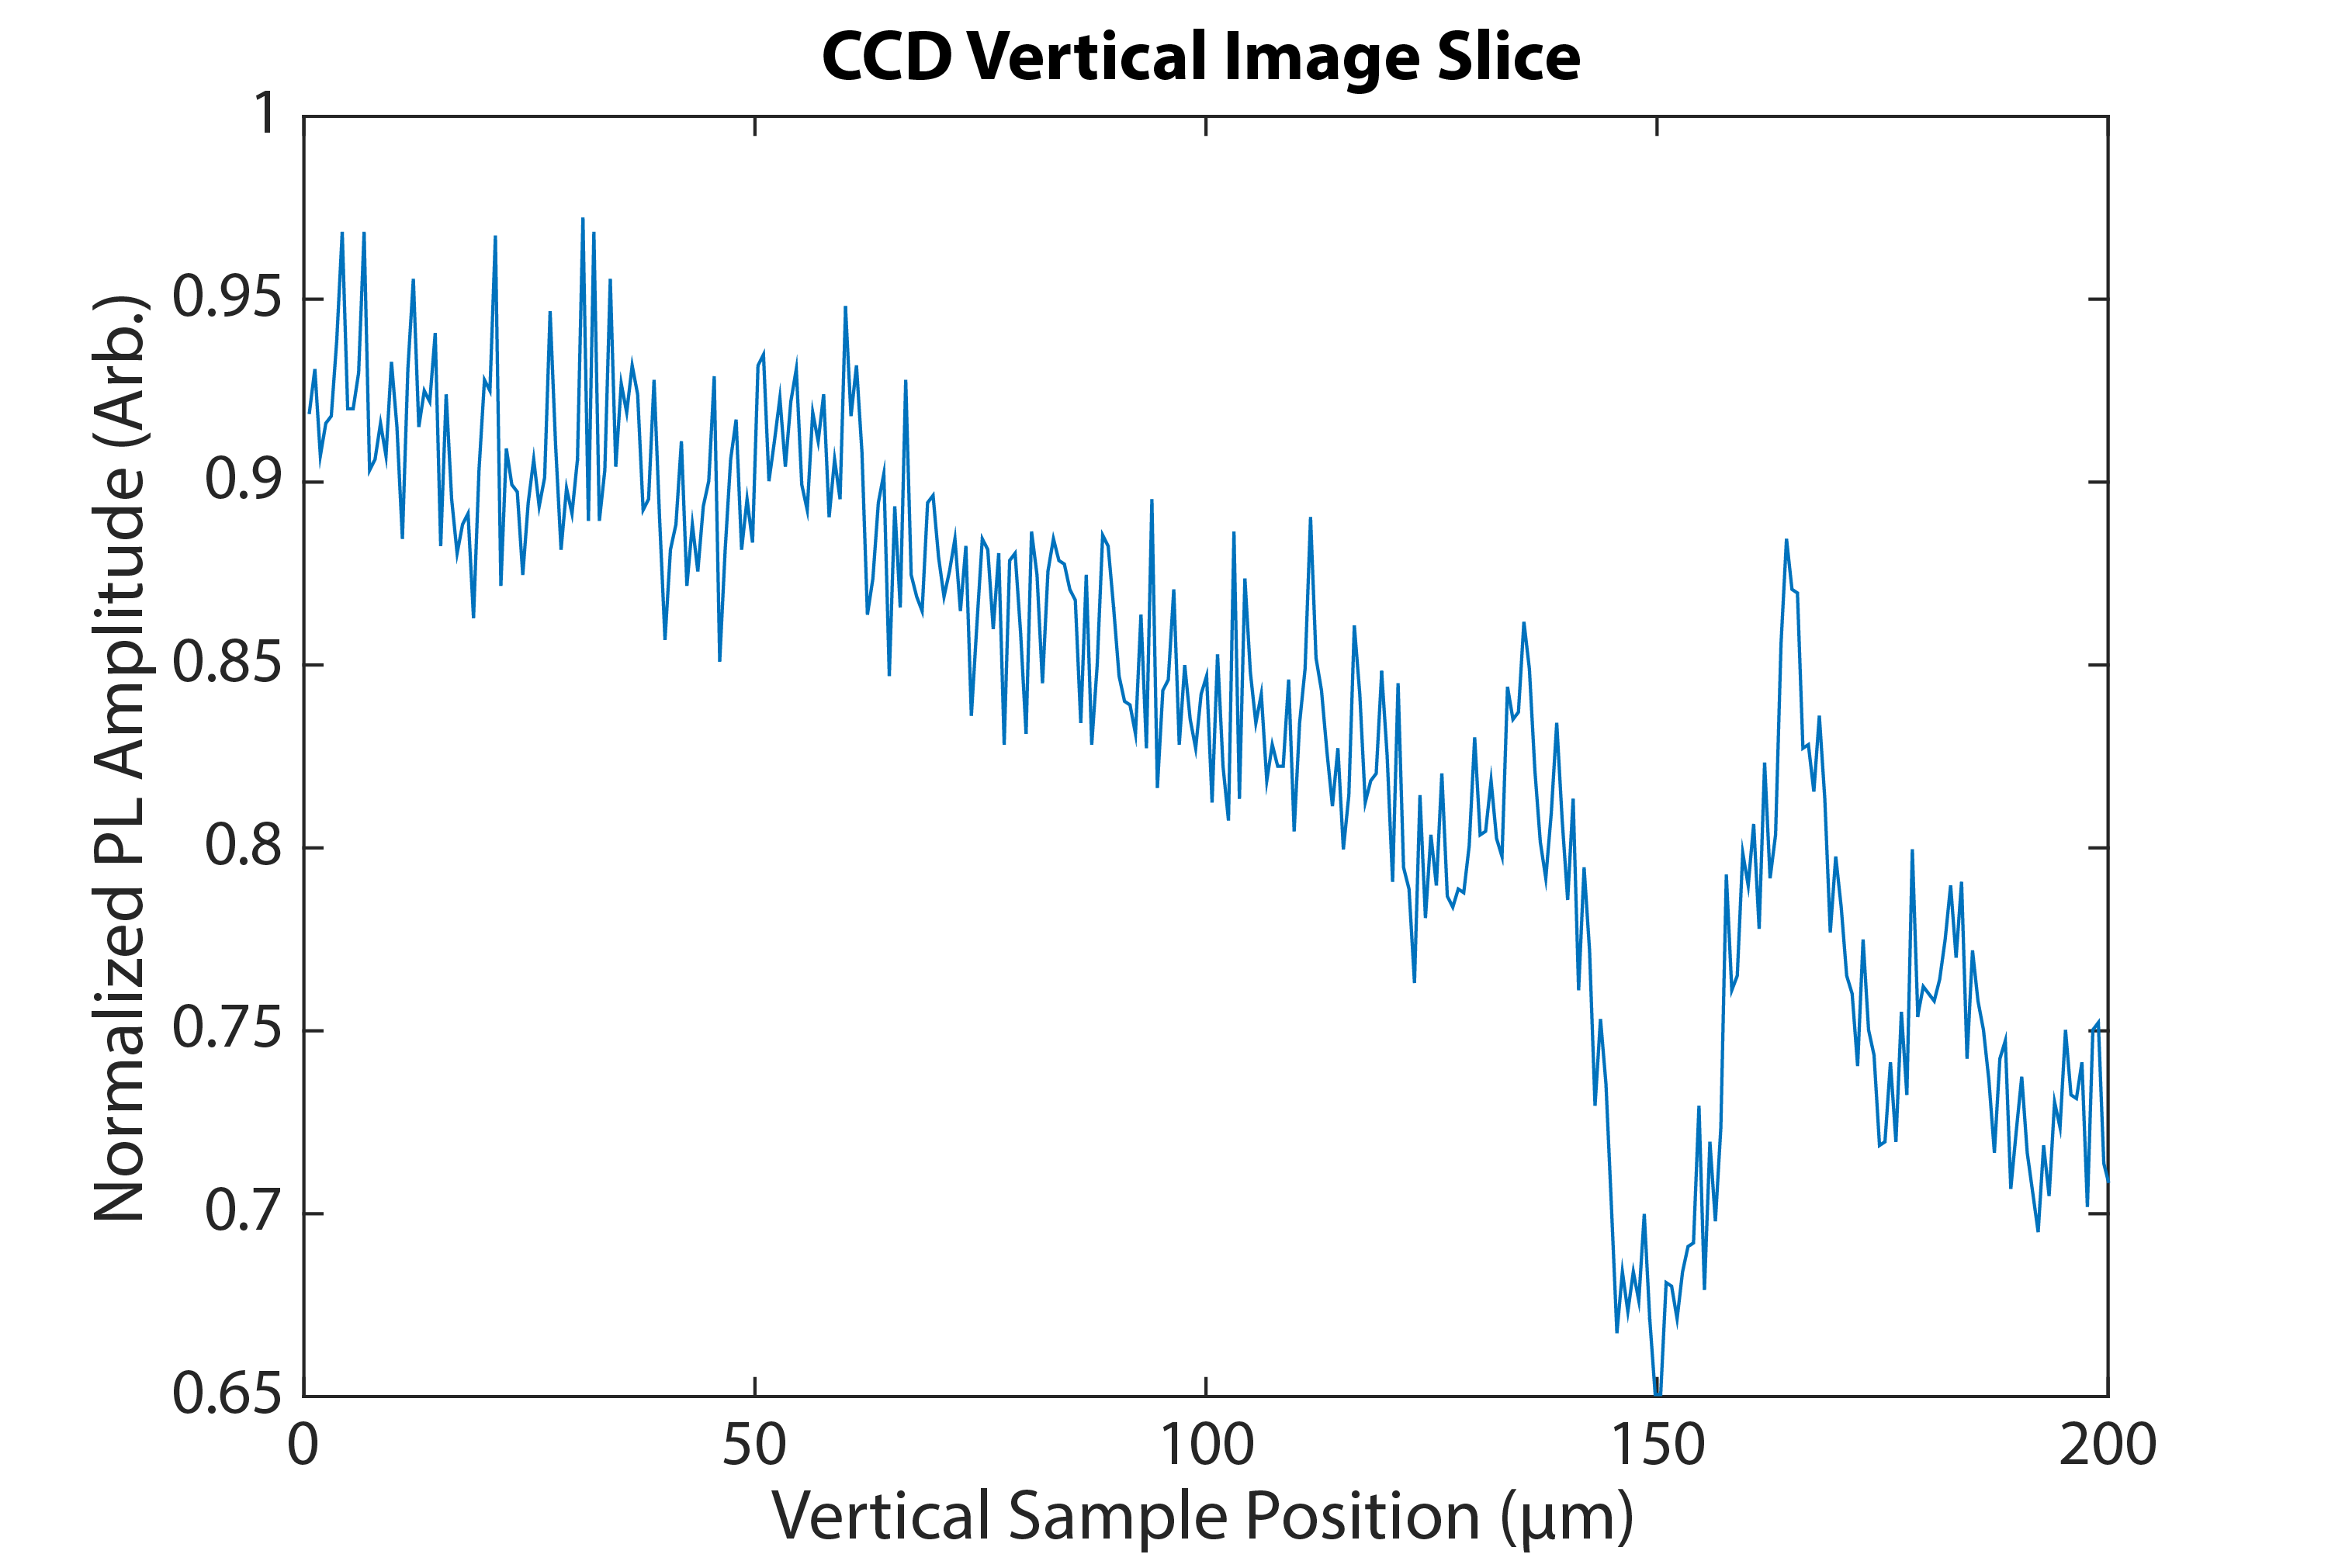
\includegraphics[width = .8\textwidth]{RawCCDIMGvertslce.png}
\caption{ \doublespacing A vertical 10QW PL amplitude slice at the PL maximum from a CCD raw image. Effectively, these slices were stacked together along the lens translation axis to recover the second sample location axis and build a 3D surface of either PL amplitude or PL energy.}
\label{slice}
\end{figure}
\begin{figure}[h!]
\centering
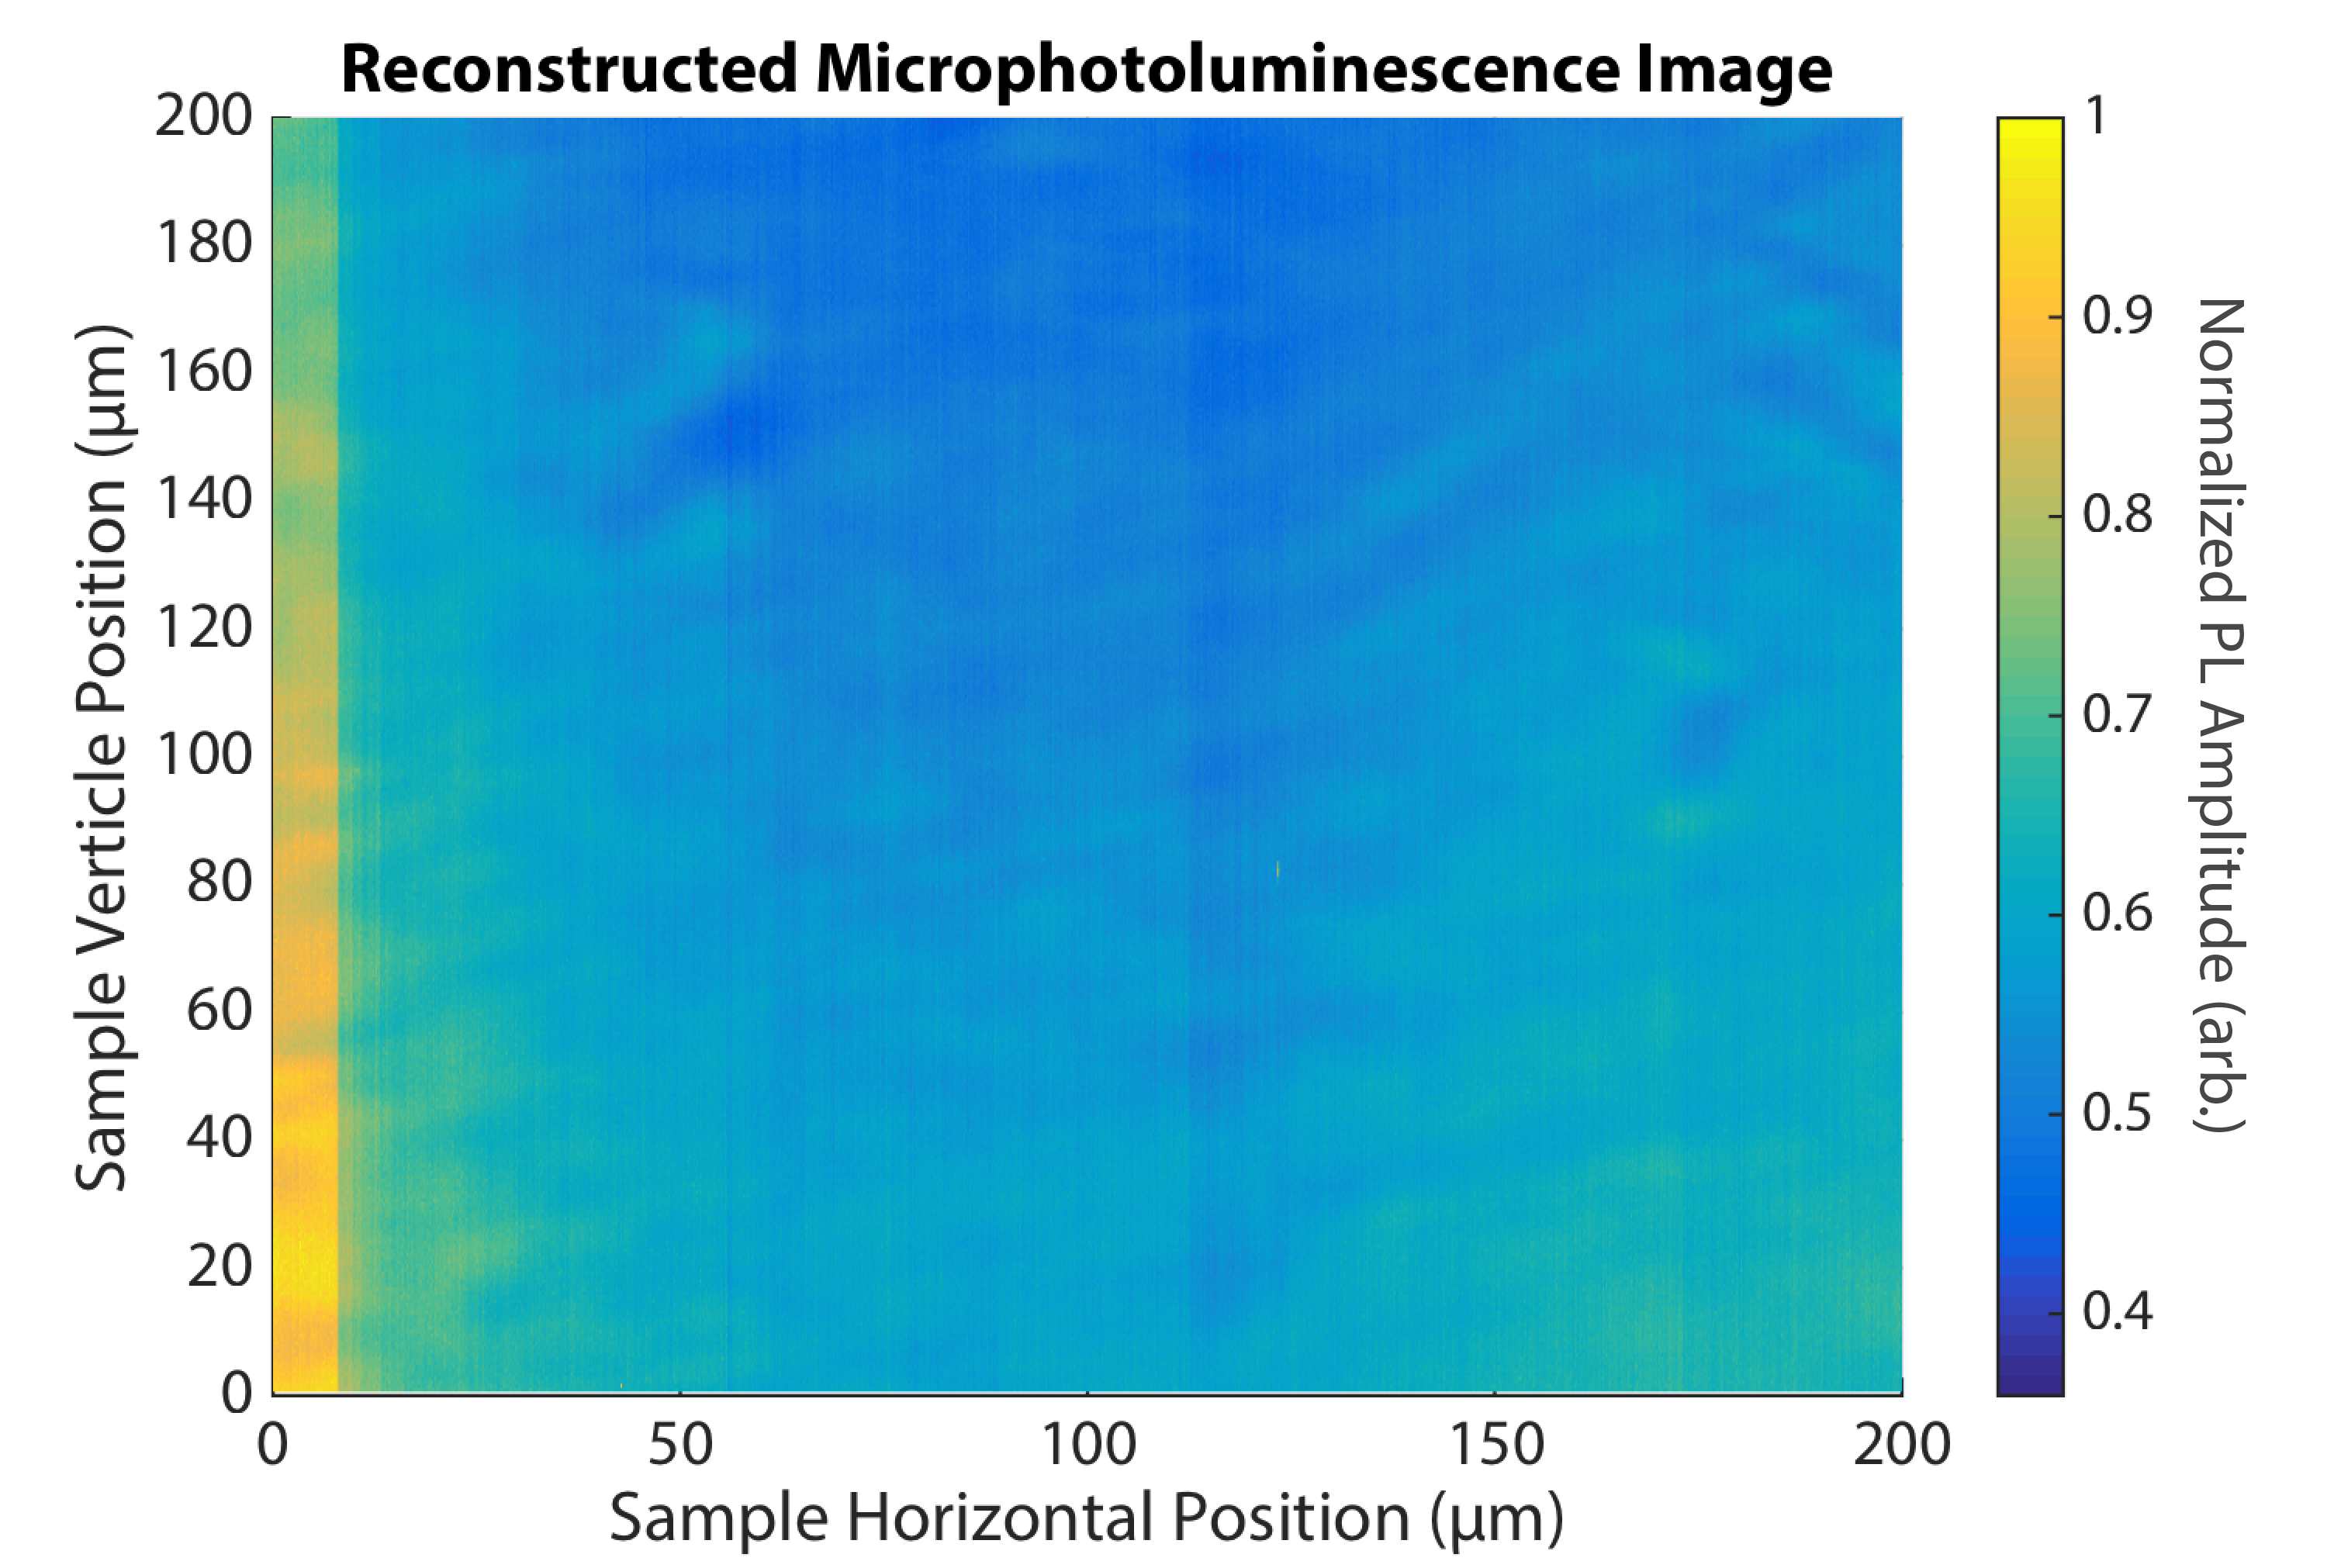
\includegraphics[width = .8\textwidth]{PLIMG_10QW.png}
\caption{ \doublespacing A reconstructed PL image of 10QW sample surface. The small features in the image correspond to striations and dust on the surface of the sample. The excitation spot's maximum intensity occurred near the bottom of the image, corresponding to the PL amplitude maximum.}
\label{total10qw}
\end{figure}
\indent From this image, we can estimate the resolution limit for the PL image alone. Doing so, we calculated that the resolution limit for our imaging system was limited by the repeatability of the lens position, $0.5\mu$m, which corresponds to 225nm at the sample surface, while we stepped the lens by slightly less than the repeatability, $0.4\mu$m, to be sure that the repeatability was the limiting factor for our horizontal resolution. We were limited in the vertical direction by the camera pixel size, which was $13.6\mu$m. Because our magnification factor was 22.22x, our vertical resolution was no better than 612nm on the sample. This was not our goal of 185nm; however, one can ameliorate this issue by inserting a telescope, with 2x magnification, between the NPBS and the achromatic doublet. An unfortunate side effect of increased resolution, however, was decreased signal strength. It was therefore necessary to increase CCD integration time or increase PL emission by increasing excitation power, but as we were exciting the sample with an already relatively high power of 1mW, increasing the resolution necessitated increasing integration time. For the 4QW sample, we took data with the telescope in place, but for the 10QW sample, a resolution of 225.0x612.0nm was the best we achieved. 
 


\indent Though our resolution was less than optimal, we were still able to calculate an energy deviation map for the 10QW sample. To do this, we found the emission energy corresponding to the maximum PL amplitude at each vertical pixel. We then stacked each of these points (for which we had an energy vs. vertical sample position vector) along the horizontal image axis at each lens position. Once done, we then calculated the average PL energy for the entire PL image. Then, we found the local energy deviation from the average PL energy by subtracting the average PL energy from the local PL energy. Simply: 
\begin{equation}
\delta E_{i,j} = E_{i,j}-E_{avg}
\end{equation}
where $E_{avg}$ is the average emission energy for the whole PL picture, and $i,j$ index horizontal and vertical sample position respectively. Following this, we obtain our $\mu$PL map. However, this map is too noisy to see structure, as CCD intensity fluctuations of roughly 10 counts or 1\% of the total signal will affect PL peak amplitude location on the CCD, and thus the peak energy at a given sample location. Therefore, we must take our $\mu$PL energy deviation map and Gaussian smooth the energy deviation values by two to five pixels FWHM depending on the sample. Doing so, we obtain the energy deviation map seen in Figure \ref{devmap10QW}. This, however, reduces our resolution further, as adjacent pixels now carry information about the average value of pixels around them. Our horizontal resolution for the deviation map, as measured on the deviation image by looking at closest distinguishable pixels, is now 360nm. Note: since we had much many more horizontal image slices than vertical pixels, the effect of the Gaussian blur on reduced resolution seemed to be more prominent in the horizontal direction. Therefore, even though adjacent pixels were still distinguishable in the vertical direction, our vertical resolution was now between 612nm and 800nm. 

\begin{figure}[h!]
\centering
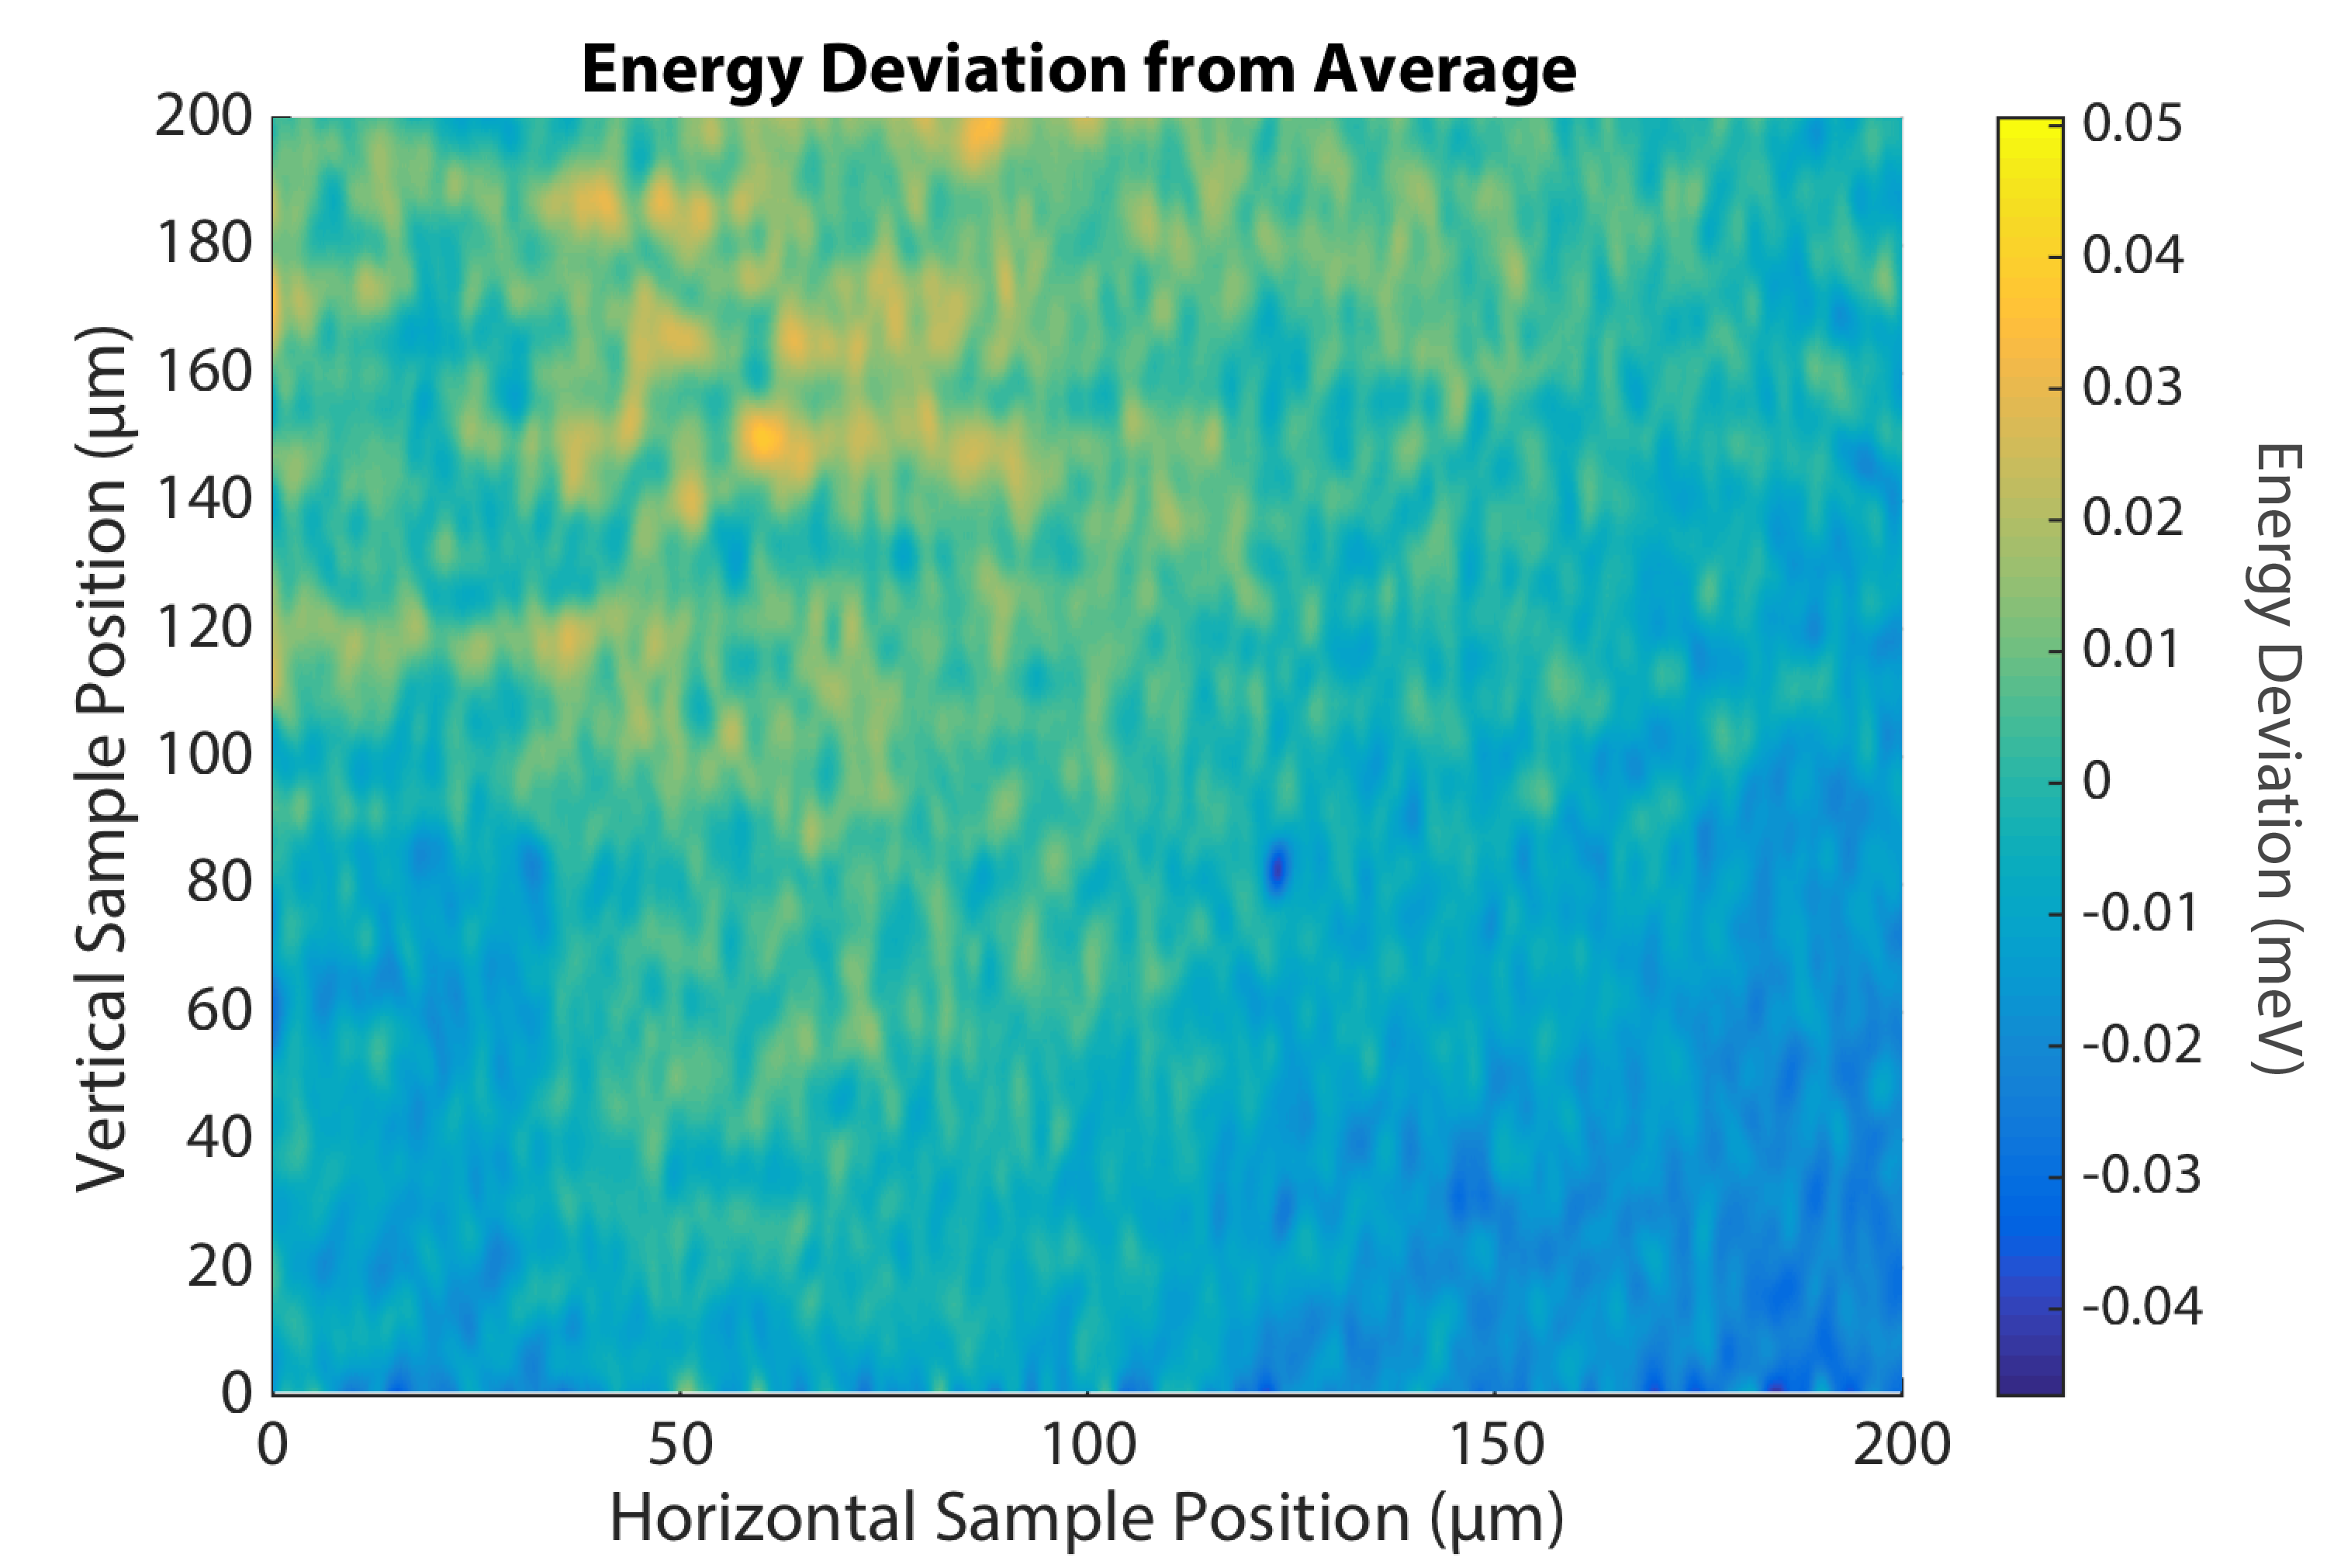
\includegraphics[width = .8\textwidth]{10QW_devplot.png}
\caption{ \doublespacing A $\mu$PL energy deviation image for the 10QW sample. Note the energy deviation was found to be 0.1meV, peak to peak, at maximum.}
\label{devmap10QW}
\end{figure}

\newpage
\indent We expected energy deviations as a result of QW width fluctuations to behave according to the following equation:
\begin{equation}
\label{de}
\delta E = \frac{h^2 \pi^2}{2 \mu_{HH}}\Big ( \frac{1}{(L^* \pm a)^2}- \frac{1}{L^{*^2}} \Big )
\end{equation}
where $\delta E$ is the PL energy deviation due to a well width fluctuation of $\pm a$, $\mu_{HH}$ is the heavy-hole reduced mass, and $L^* = L+2\delta$ is the effective well width accounting for electron wave-function penetration of $15$\AA ~ into the AlGaAs barrier, and $\mu_{HH} = 0.055m_e$ is the reduced exciton mass \cite{glinka, santos}. We saw energy deviations of about \ref{0.1}meVpp, which was five times less than expected. This discrepancy was due for the most part to signal averaging within the 10QW sample PL image: the relatively weak PL signal from spots in the wells which deviated from average width was most likely from the first few wells, and not all 10QWs. Additionally, since we looked only at the maximum amplitude PL signal from each point in the sample, due to the random distribution of disorder, the maximum PL energies at each PL image location would tend to be close to the average PL energy for the whole sample, as the signal at each location was presumably an average over the QW emission from each well at each imaging location. In other words: the way we took our PL image meant that any disorder deviations we saw would be due to the additive effects of disorder over multiple wells, meaning that disorder fluctuations were smaller than expected in the one QW limit. Using Equation 4.2, we expect energy deviations of roughly 0.5meV for disorder variations of one crystal monolayer. Anything less than this corresponds to no measured well width variations whatsoever. However, we do measure energy deviations in our $\mu$PL images. What we are measuring is the averaged width fluctuations over a number of quantum wells, not width fluctuations for just one well.



\subsection{Disorder in a Four Quantum Well Structure}
Because the 10QW PL energy deviations due disorder were fairly small, we decided to take $\mu$PL data on a four-period 10nm GaAs QW with 10nm AlGaAs barriers. As 4QW sample had fewer wells, but each was identical in width to the 10QW sample, we expected to see larger disorder energy deviations because there would be fewer wells over which the signal would be averaged. Additionally, we inserted a telescope into the PL imaging path, increasing our on-sample resolution. In the horizontal direction, the resolution limit was no longer set by the lens translation. Rather, since we were able to magnify our image by 2x, the horizontal resolution was diffraction limited to $192.9\pm0.3$ nm, as our PL wavelength peaked around 807.8nm, with a FWHM of 0.6nm. The vertical resolution was increased by a factor of two from 612.0nm to 306.0nm. Therefore, for the 4QW sample, our on-sample resolution was theoretically 192.9x306.0nm. This is close to our goal of a completely diffraction-limited system, but we still weren't quite able to achieve that in the vertical imaging direction. However, again the energy deviation map data was quite noisy. As a result, we Gaussian smoothed the data with a FWHM of 2px at each data point. Therefore, though our PL image had a resolution of 192.9x306.0, our energy 4QW map was limited to a resolution of 252x400nm. Figure \ref{4qwimg} is a reconstructed PL image collected from the 4QW sample, while figure \ref{4qwdev} is the image deviation map corresponding to the PL image. 
\newpage
\begin{figure}[h!]
\centering
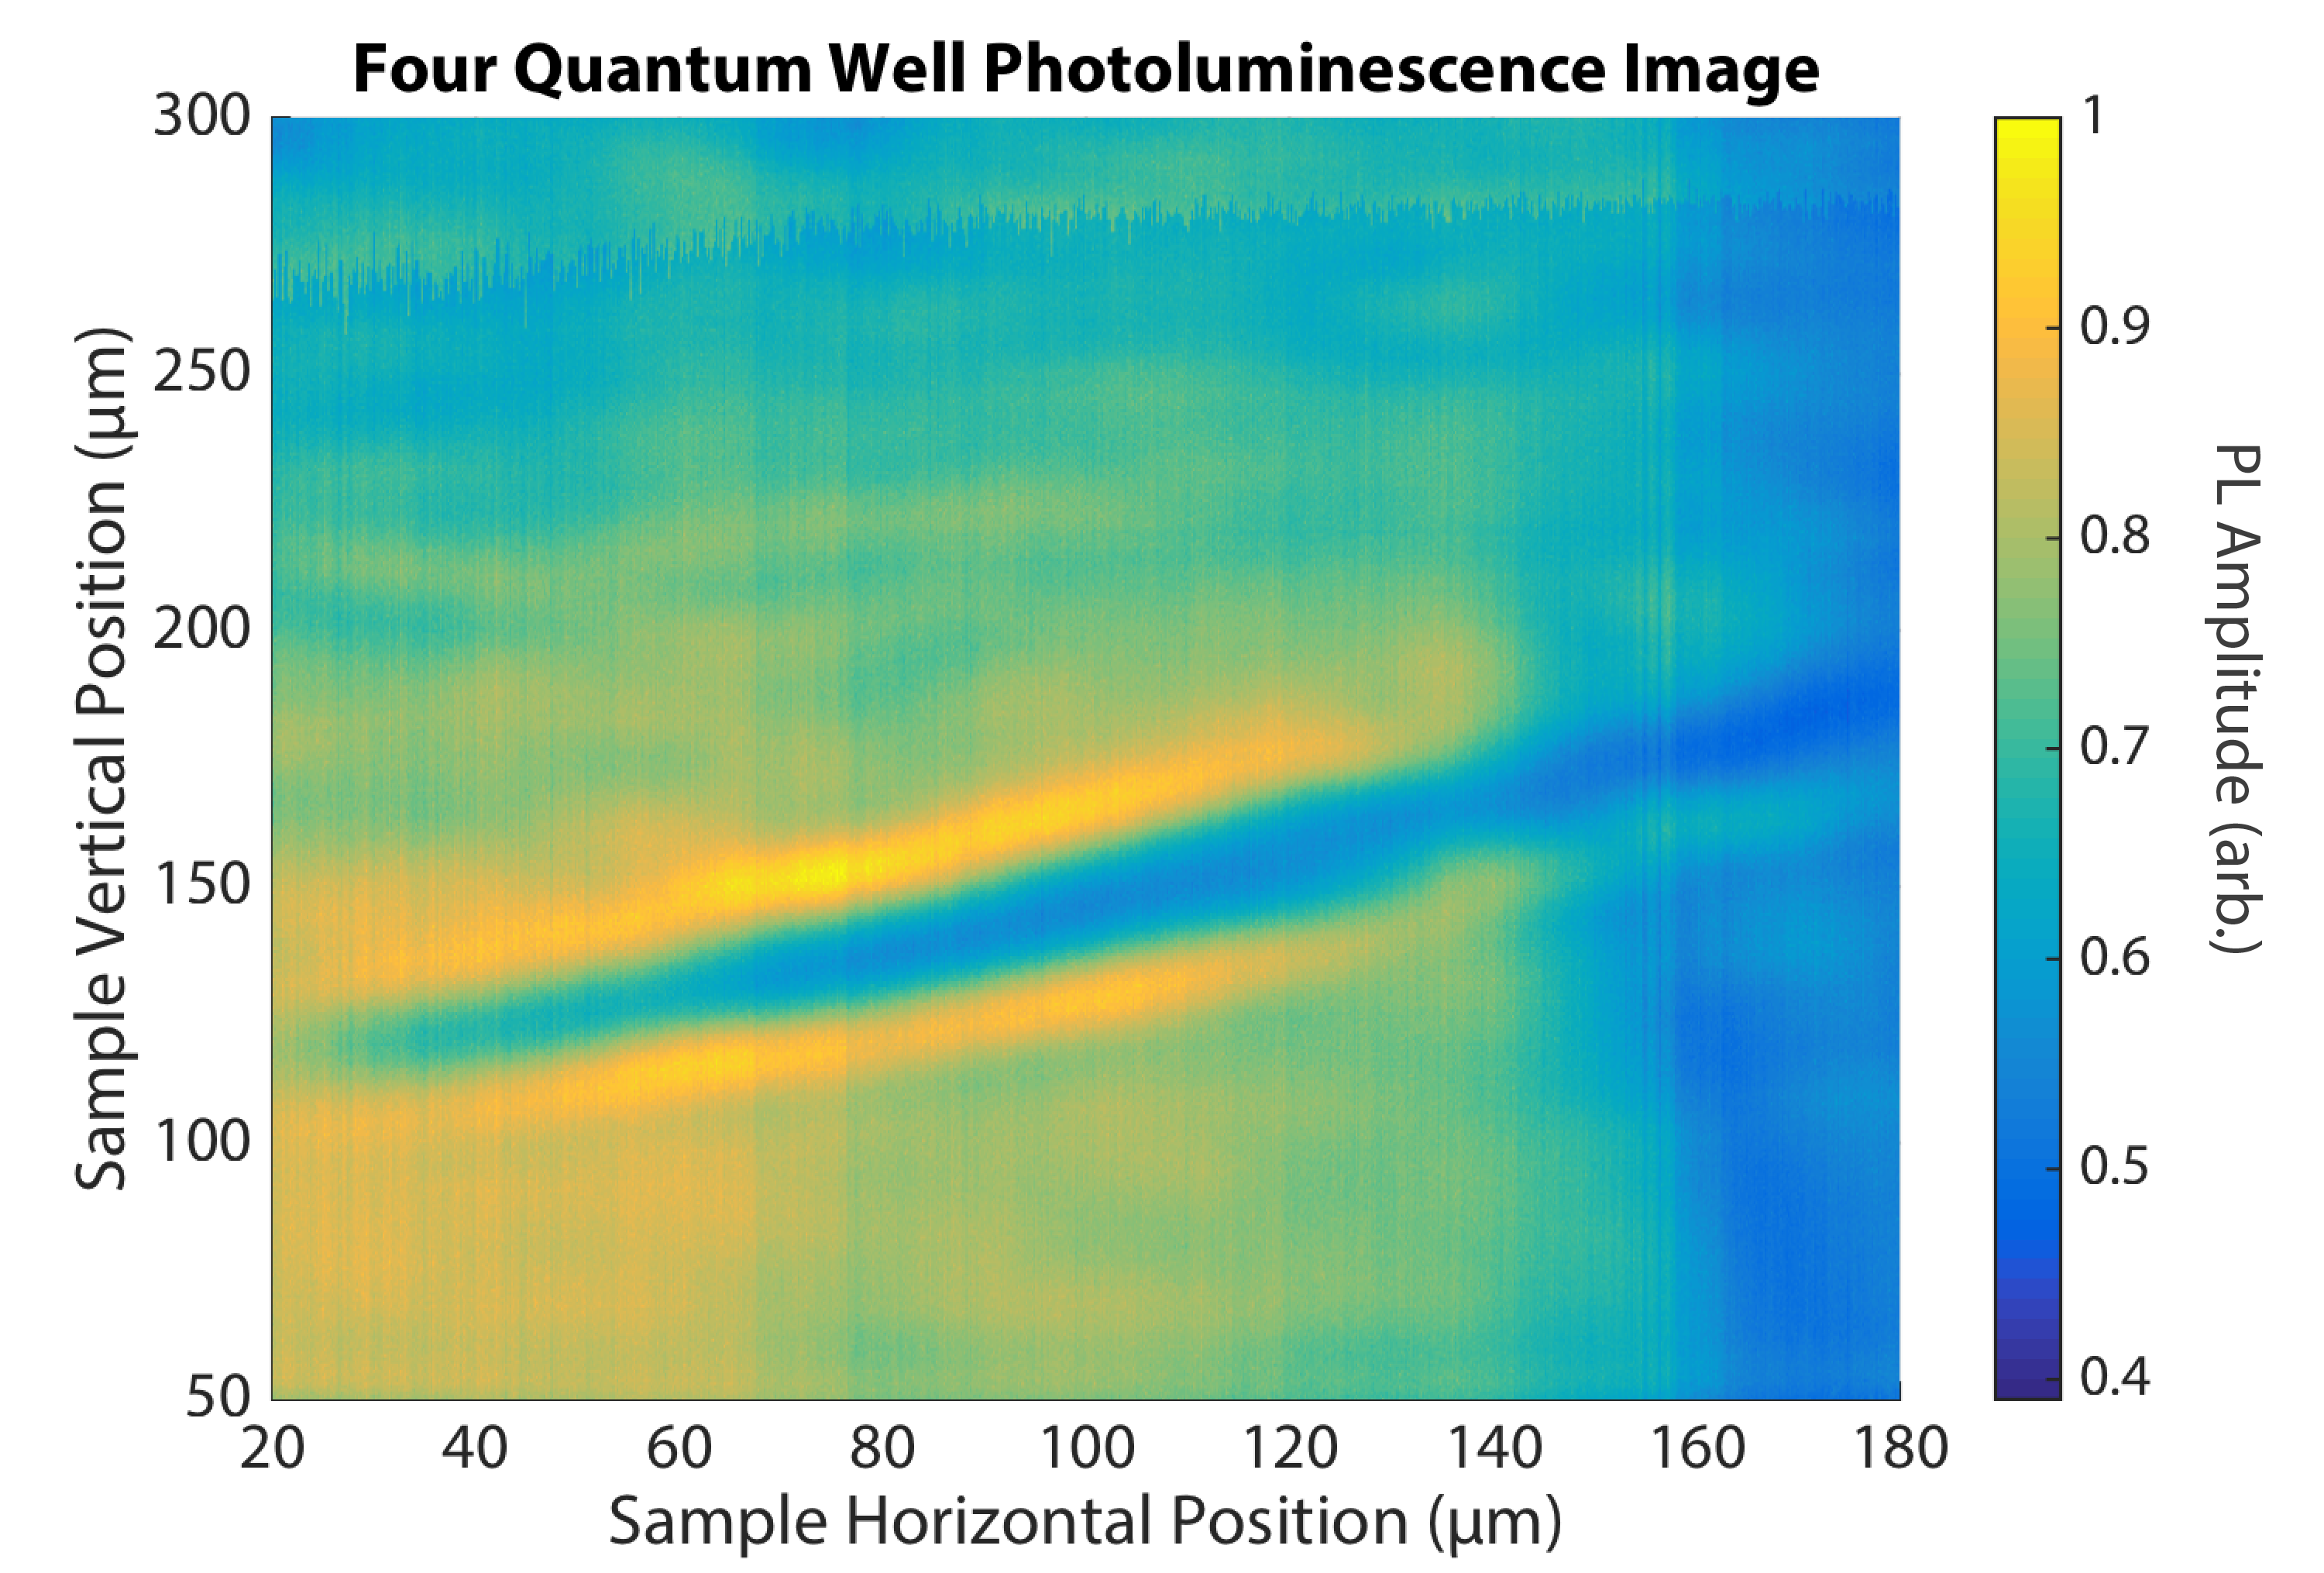
\includegraphics[width = .6\textwidth]{4QW_Img.png}
\caption{ \doublespacing A reconstructed image of the PL amplitude of the 4QW sample.}
\label{4qwimg}
\end{figure}
\begin{figure}[h!]
\centering
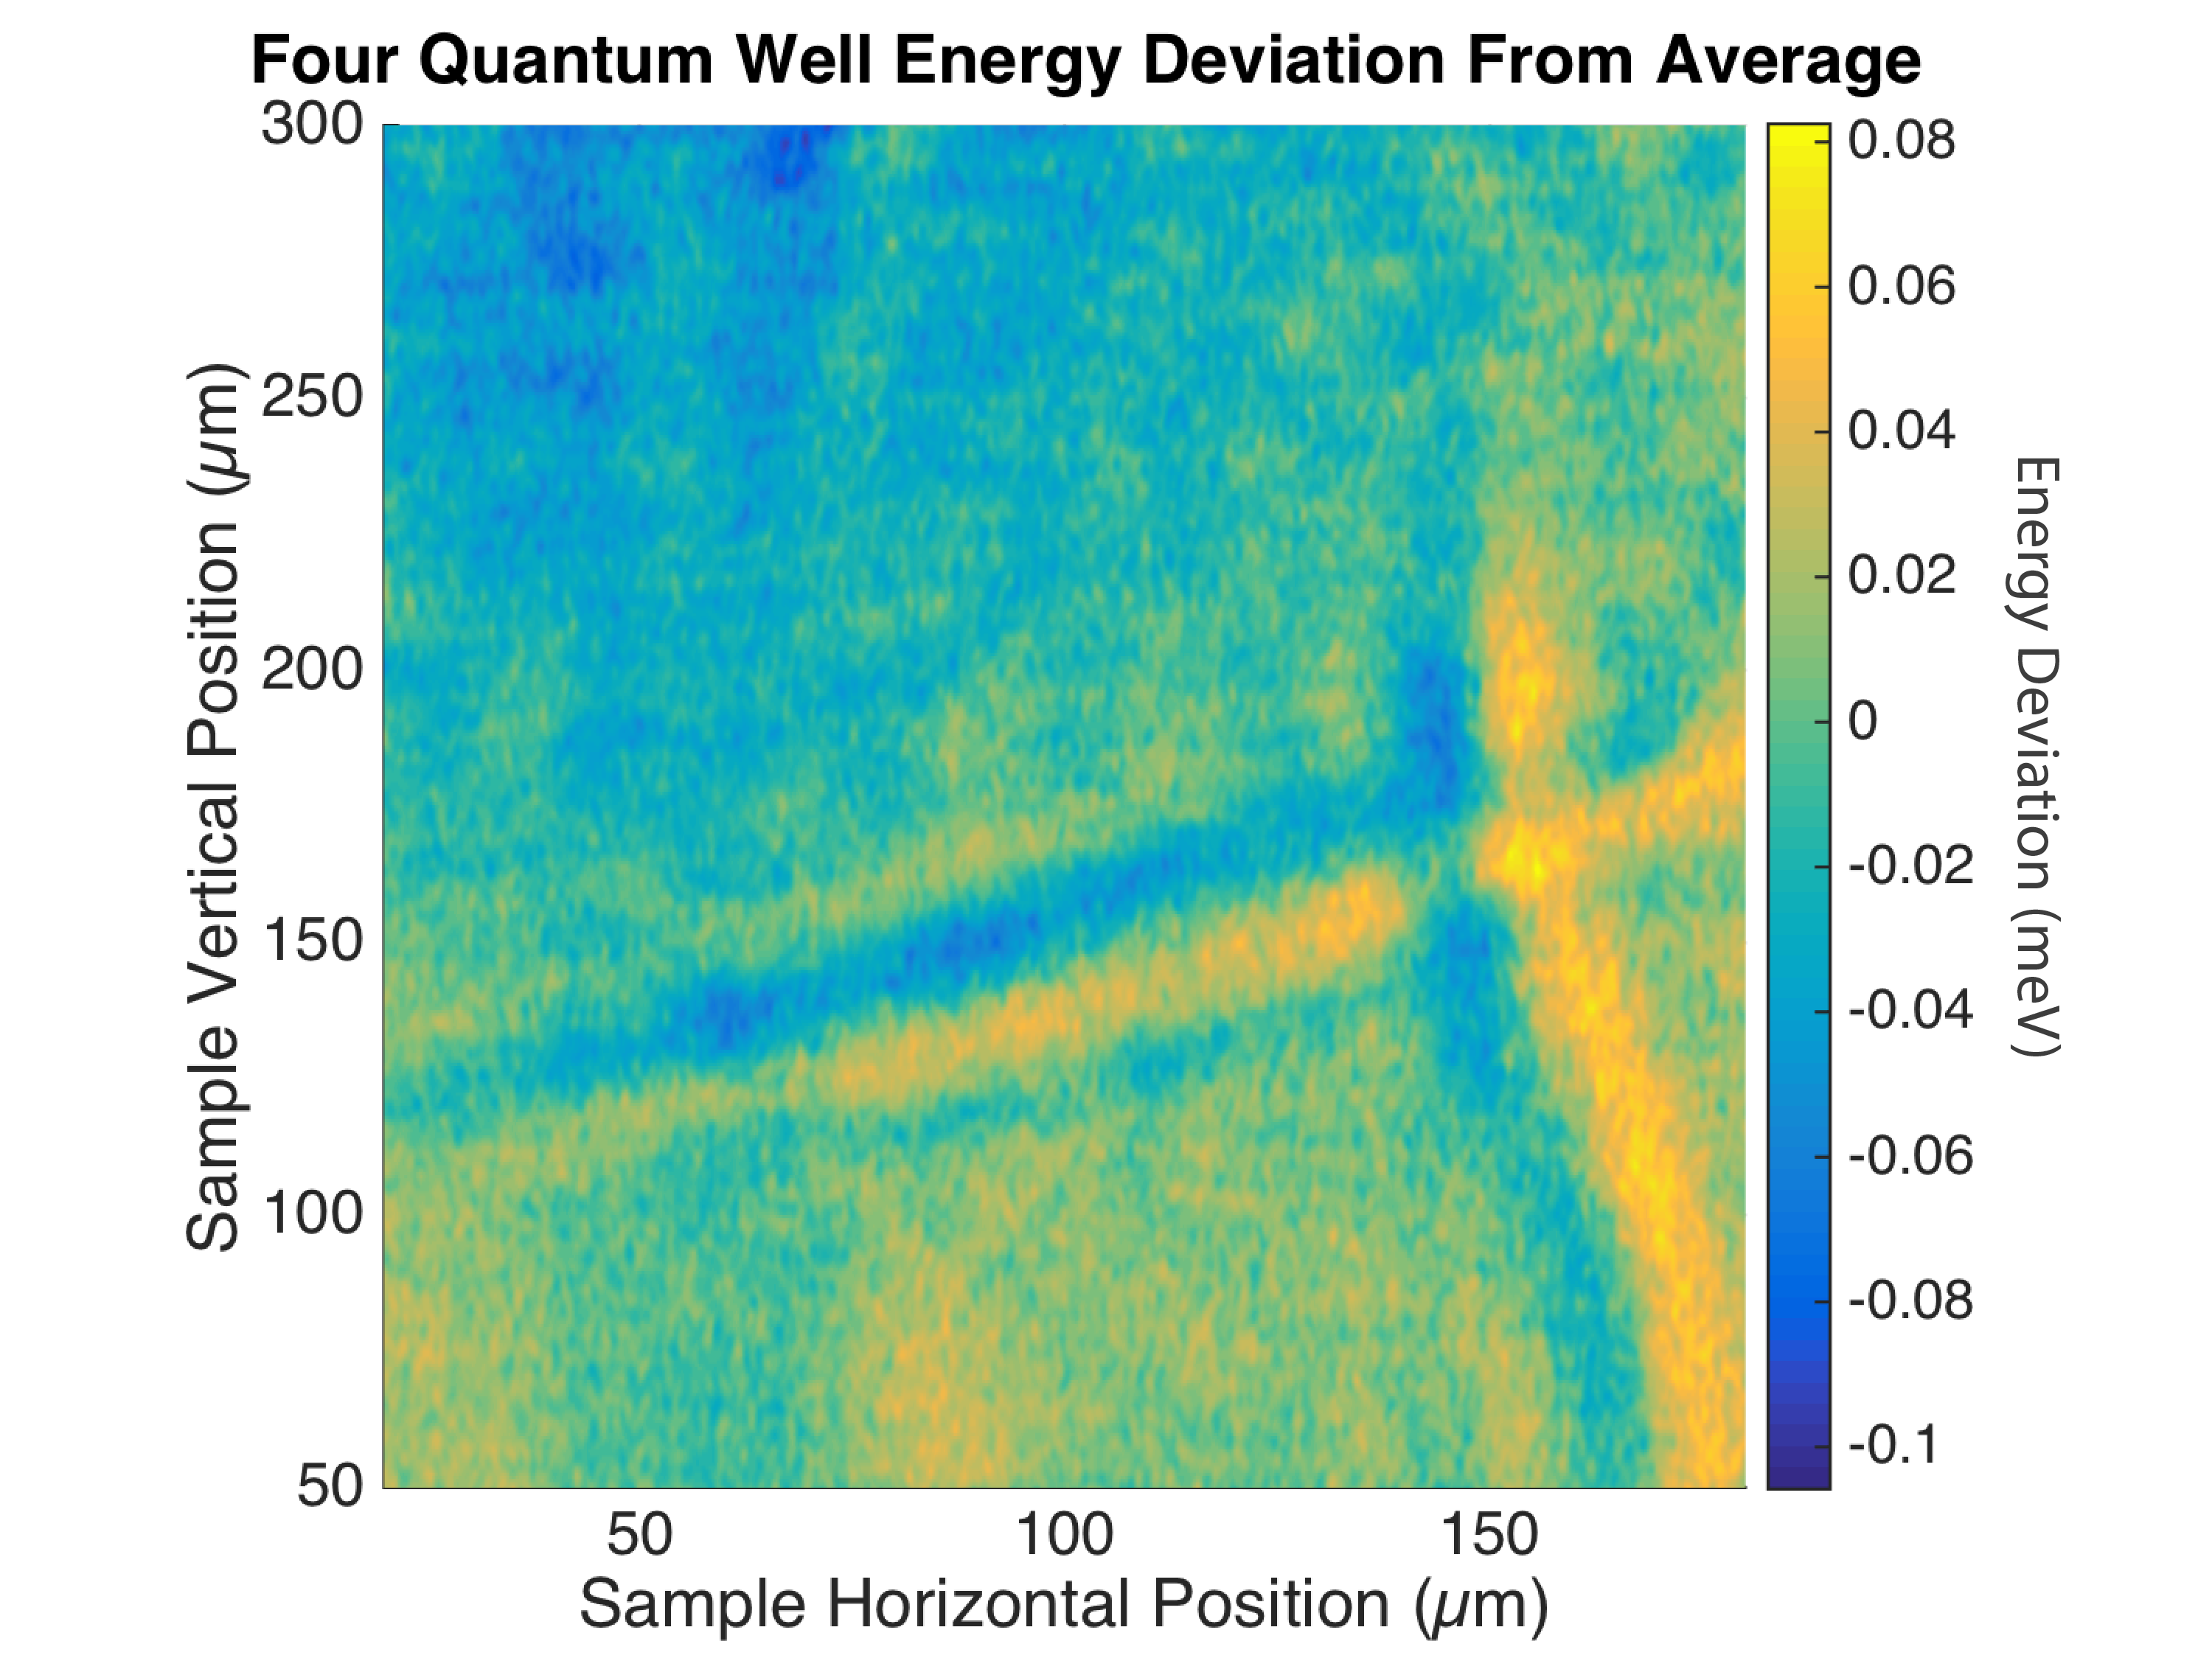
\includegraphics[width = .7\textwidth]{4QW_devplot.png}
\caption{ \doublespacing An energy deviation map for the 4QW sample. Note the large-scale feature across the middle of the sample. This most likely corresponded to a scratch across the sample which slightly deformed all four wells below it, so we see an energy signature of this deformation.}
\label{4qwdev}
\end{figure}
\newpage

\indent With the periodic 4QW structure, we were still running into the same problems we had with the 10QW sample: due to spectral averaging over multiple quantum wells, we saw energy deviations corresponding to well width variations of less than a monolayer. Though the energy deviations from disorder for each single quantum well were presumably larger than those we saw, we weren't able to resolve the disorder variations in just one quantum well. 

\subsection{Disorder in an Interfacial Quantum Dot Structure}
\indent Our final disorder measurement was taken on an interfacial quantum dot (IQD) sample. Due to high signal averaging for the MQW samples, we weren't able to see the energy deviations we theoretically should have. Subsequently, we took $\mu$PL data on a 5-period, varying well and barrier thickness GaAs/AlGaAs quantum well. Due to the growth process of the IQD sample, smaller well widths and similar width fluctuations translate to three-dimensional exciton confinement \cite{galanthesis, fox}, rather than just the one QW confinement dimension. Though the sample was a five-period structure, there was less spectral averaging than the 10QW and 4QW samples. This is clear in Figure \ref{iqdDev}. Additionally, due to the smaller well width for some of the IQD wells relative to the other two QW samples, our original light source was slightly unreliable at the shorter wavelengths necessary to probe IQD disorder: as we tuned the Ti:Sapph laser below 750nm, it would occasionally enter multi-mode operation. When this occurred, the laser would operate at diminished and unstable power. We therefore used a green laser, centered at 532.15nm to excite the IQD sample.


\begin{figure}
\centering
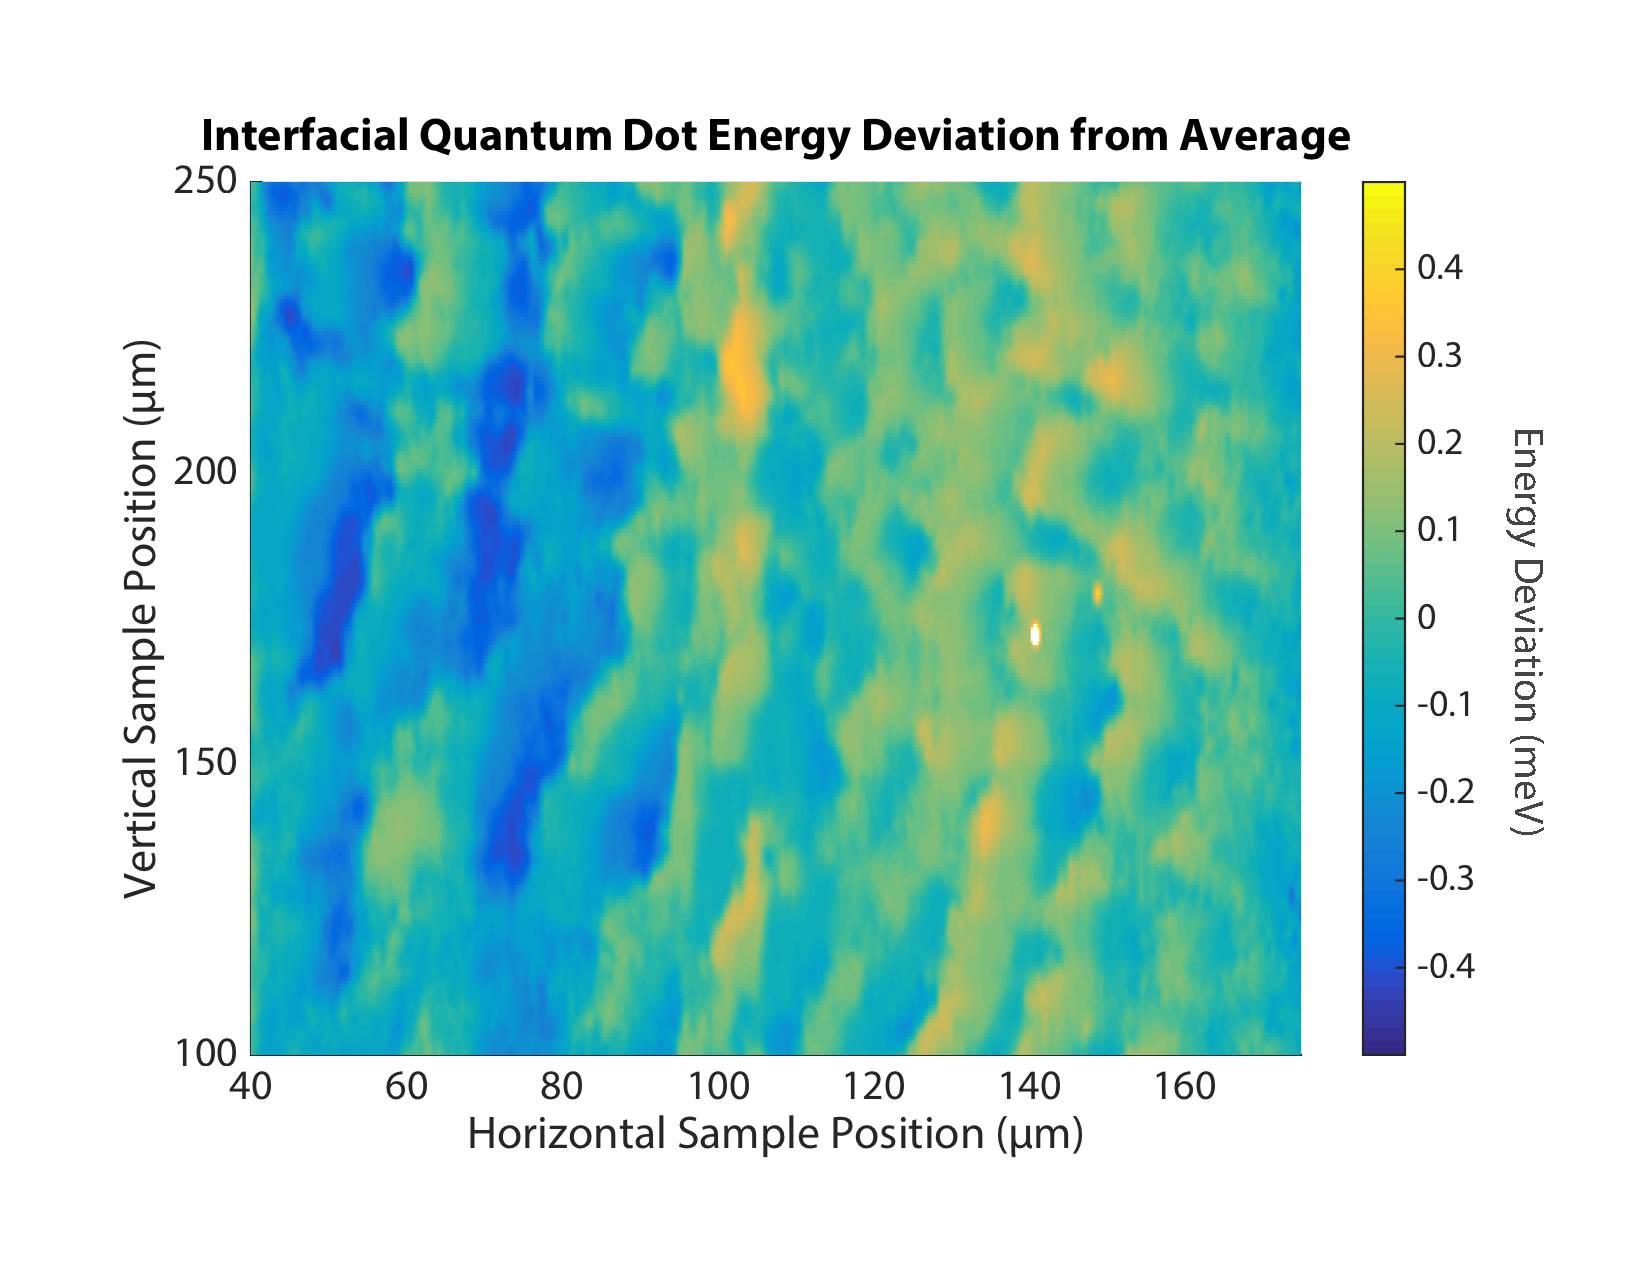
\includegraphics[width = .9\textwidth]{iqd2.pdf}
\caption{ \doublespacing An energy deviation map for the IQD sample. The energy deviations in the IQD sample are much larger than those measured in the 4QW and 10QW samples, even though the IQD structure is periodic and suffers from similar spectral averaging to the other samples. The white blemish is an anomalous noise spike.}
\label{iqdDev}
\end{figure}
\indent From these measurements, we were able to calculate a maximum PL energy deviation of 0.74meV, peak to peak. This value was larger (and much more representative of PL energy fluctuations caused by disorder) than that for 10QW and 4QW structures. Therefore, we were able to measure well width variations greater than one monolayer in the IQD sample. Though there was still spectral averaging due to the fact that the IQD sample was five wells thick, this was due to the diversity of well widths present in the IQD sample by design.


\section{PLE Results and Analysis}
\indent For our asymmetric double quantum well samples, we had InGaAs wells of 9nm and 10nm thickness with a GaAs barrier between them. We had three samples of varying barrier thickness, b, with $b=5,10,$ or $30$nm. For each sample, we excited with our CW laser, and collected PL from the sample. We then stepped our laser excitation wavelength and monitored the PL spectra as a function of CW excitation wavelength. We found in each case that there was incoherent Stokes- and anti-Stokes coupling of excitons between wells. Figure \ref{peakscheme} shows a close-up of the coupling peaks, while Figure \ref{scan} shows an example PLE spectrum for an AQW sample with a barrier width of 10nm. 



\indent Traditionally, PLE is done by monitoring emission intensity at a single wavelength \cite{borri}, but with our experiment, we are able to measure a full spectrum at each excitation wavelength. This ability means that our PLE spectra are more rich, as they provide simultaneous information of both narrow and wide well emission. Taking vertical slices along the emission peaks from the narrow and wide wells, we obtain information on exciton population by monitoring the emission amplitudes. We can then plot PLE emission amplitude as a function of excitation wavelength and monitor the strength of the Stokes- and anti-Stokes cross peaks as well as other peaks in emission corresponding to exciton ground and excited state emission. Figure \ref{traces} is an assembly of vertical PLE slices for three PLE spectra recorded at 10K. Note: as the barrier width decreases, the strength of the Stokes- and anti-Stokes peaks increases. 



\indent Figure \ref{traces} shows increased coupling between wells as barrier width decreases: both the red dashed trace peak around 1.46eV and the blue trace peak around 1.47eV increase as barrier width decreases. We measure, then, what we expect qualitatively: as AQWs get closer together, the incoherent coupling between excitons in each well increases. However, we were initially surprised that we measured coupling in the anti-Stokes direction. Intuitively, one would expect that an exciton in the wider well, because it exists at a slightly lower energy, would not be able to emit from a state in the narrower well. We suspected, therefore, that coupling in the anti-Stokes direction would be a temperature mediated process. As a result, we took PLE data on all three barrier sizes and monitored the cross-peak intensity as a function of temperature. Figure \ref{xpkintensity} shows that the coupling between wells seems to be a temperature mediated process in the 10nm and 30nm barrier samples. However, in the 5nm barrier sample, the temperature dependance of coupling seems to be vanishingly small if any, likely because the barrier acts more like a perturbation to the exciton ground state than a true well barrier. In the lower set of figures, the cross-peak intensity is normalized to the resonant peak intensity by measuring the wings of the resonant peak at three locations: on resonance, and at slightly lower and higher detection frequencies. Then, because the resonant peak was obscured by the laser scatter signal, we estimate the hight of the resonant peak using the shape and intensity of the peak wings. We then use the estimated resonant peak height to normalize the cross-peaks so we can compare the height of the cross-peaks to the height of the resonant peaks and comment on the coupling emission intensity relative to the resonant emission intensity. Others have seen similar temperature-dependence of coupling in the anti-Stokes direction, \cite{borri} but have failed to provide a model that accounts for the intensity of the coupling peaks as a function of temperature and of barrier width. 
\begin{figure}
\centering
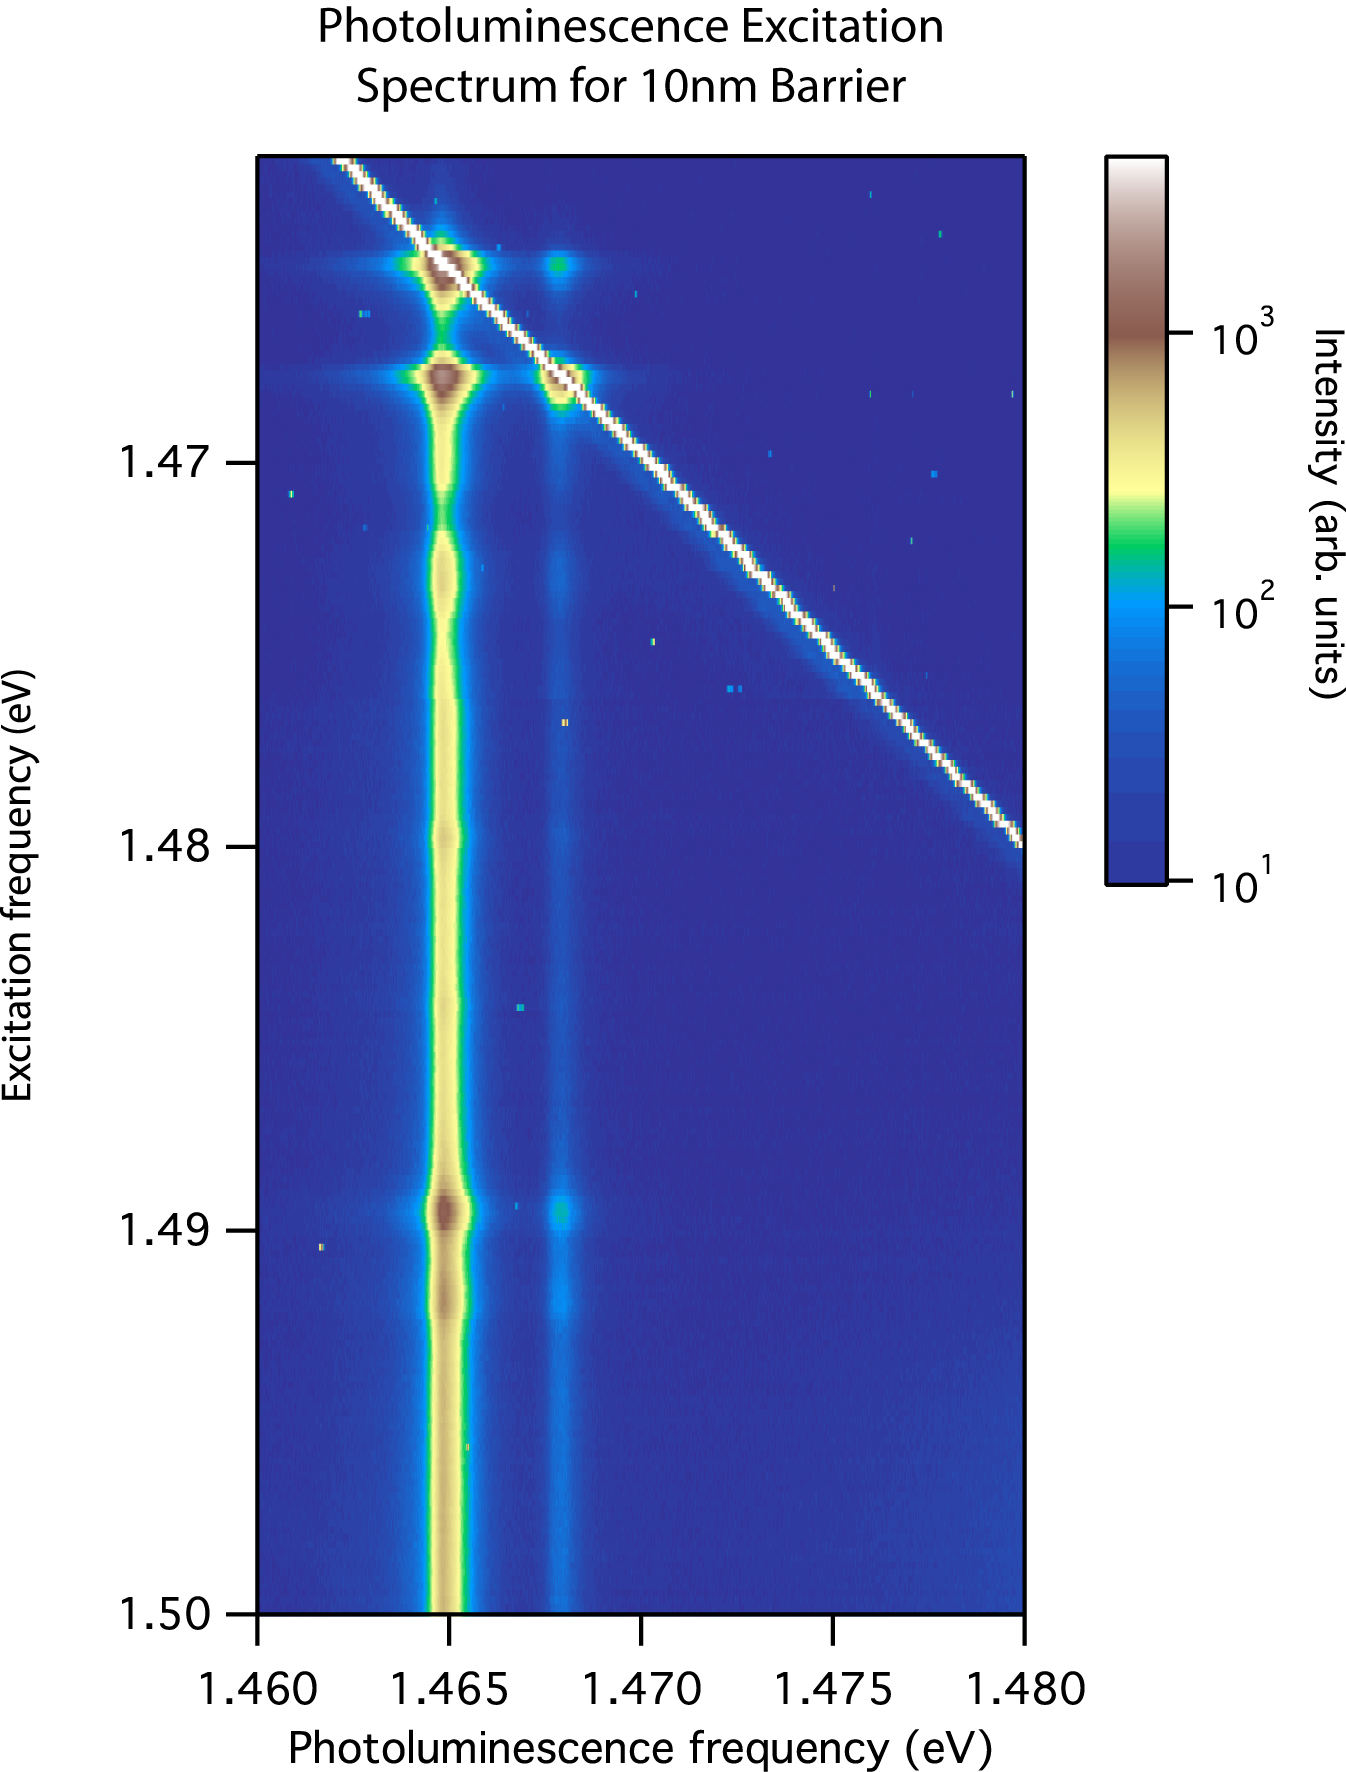
\includegraphics[width = .8\textwidth]{Layout5.jpg}
\caption{ \doublespacing An example PLE spectrum taken on a 10nm barrier AQW sample. We were able to monitor the emission from both wells as a function of excitation frequency, which allowed us to simultaneously quantify emission from one well due to resonant excitation and emission from the adjacent well due to coupling. The lower energy vertical trace corresponds to emission from the wide well while the higher energy trace corresponds to emission from the narrow well. The white diagonal line is laser scatter, and represents locations of equal excitation and detection frequencies.}
\label{scan}
\end{figure}

\begin{figure}
\centering
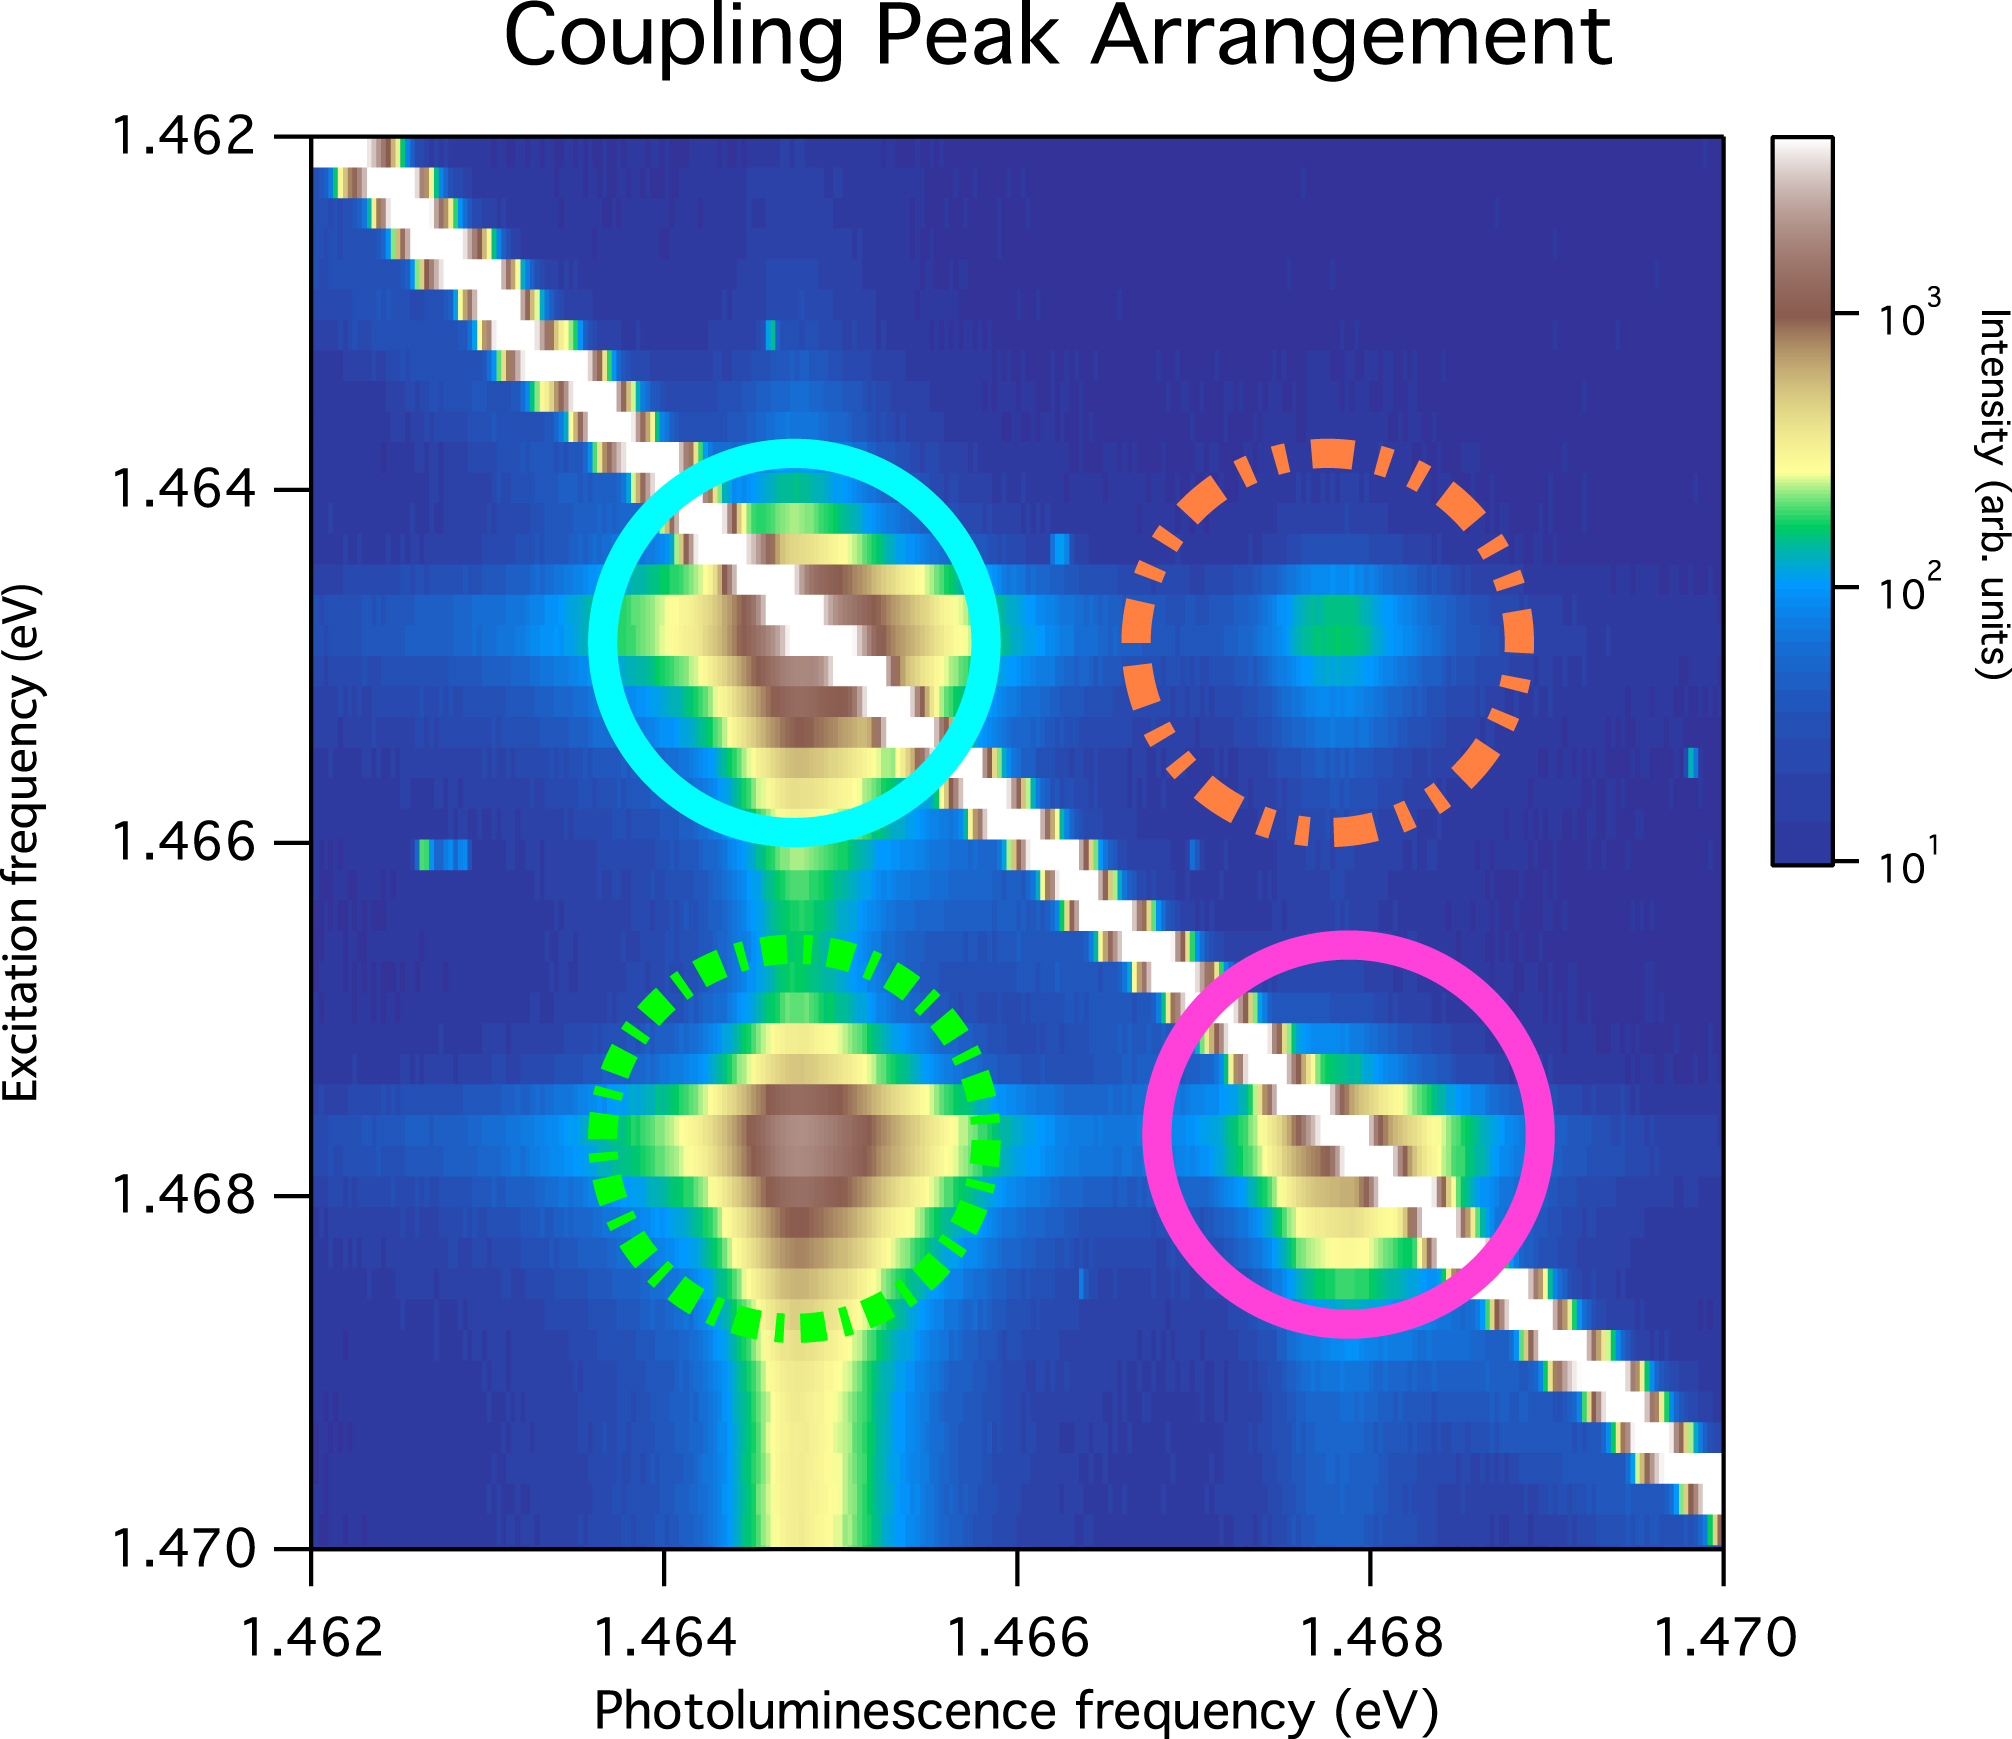
\includegraphics[width = .8\textwidth]{Layouttryit.jpg}
\caption{ \doublespacing A close-up of the coupling cross-peaks. The green, dashed circle corresponds to a coupling peak between wells in the Stokes direction: the narrow well absorbs the laser excitation, while the wide wells emit a portion of the absorbed energy. The orange, dashed circle corresponds to a coupling peak in the anti-Stokes direction: the wide well absorbs and the narrow well emits a portion of the excitation energy. The magenta circle corresponds to resonant excitation in the narrow well, and the turquoise circle corresponds to resonant excitation in the wide well. The diagonal white trace is the laser scatter.}
\label{peakscheme}
\end{figure}

\begin{figure}
\centering
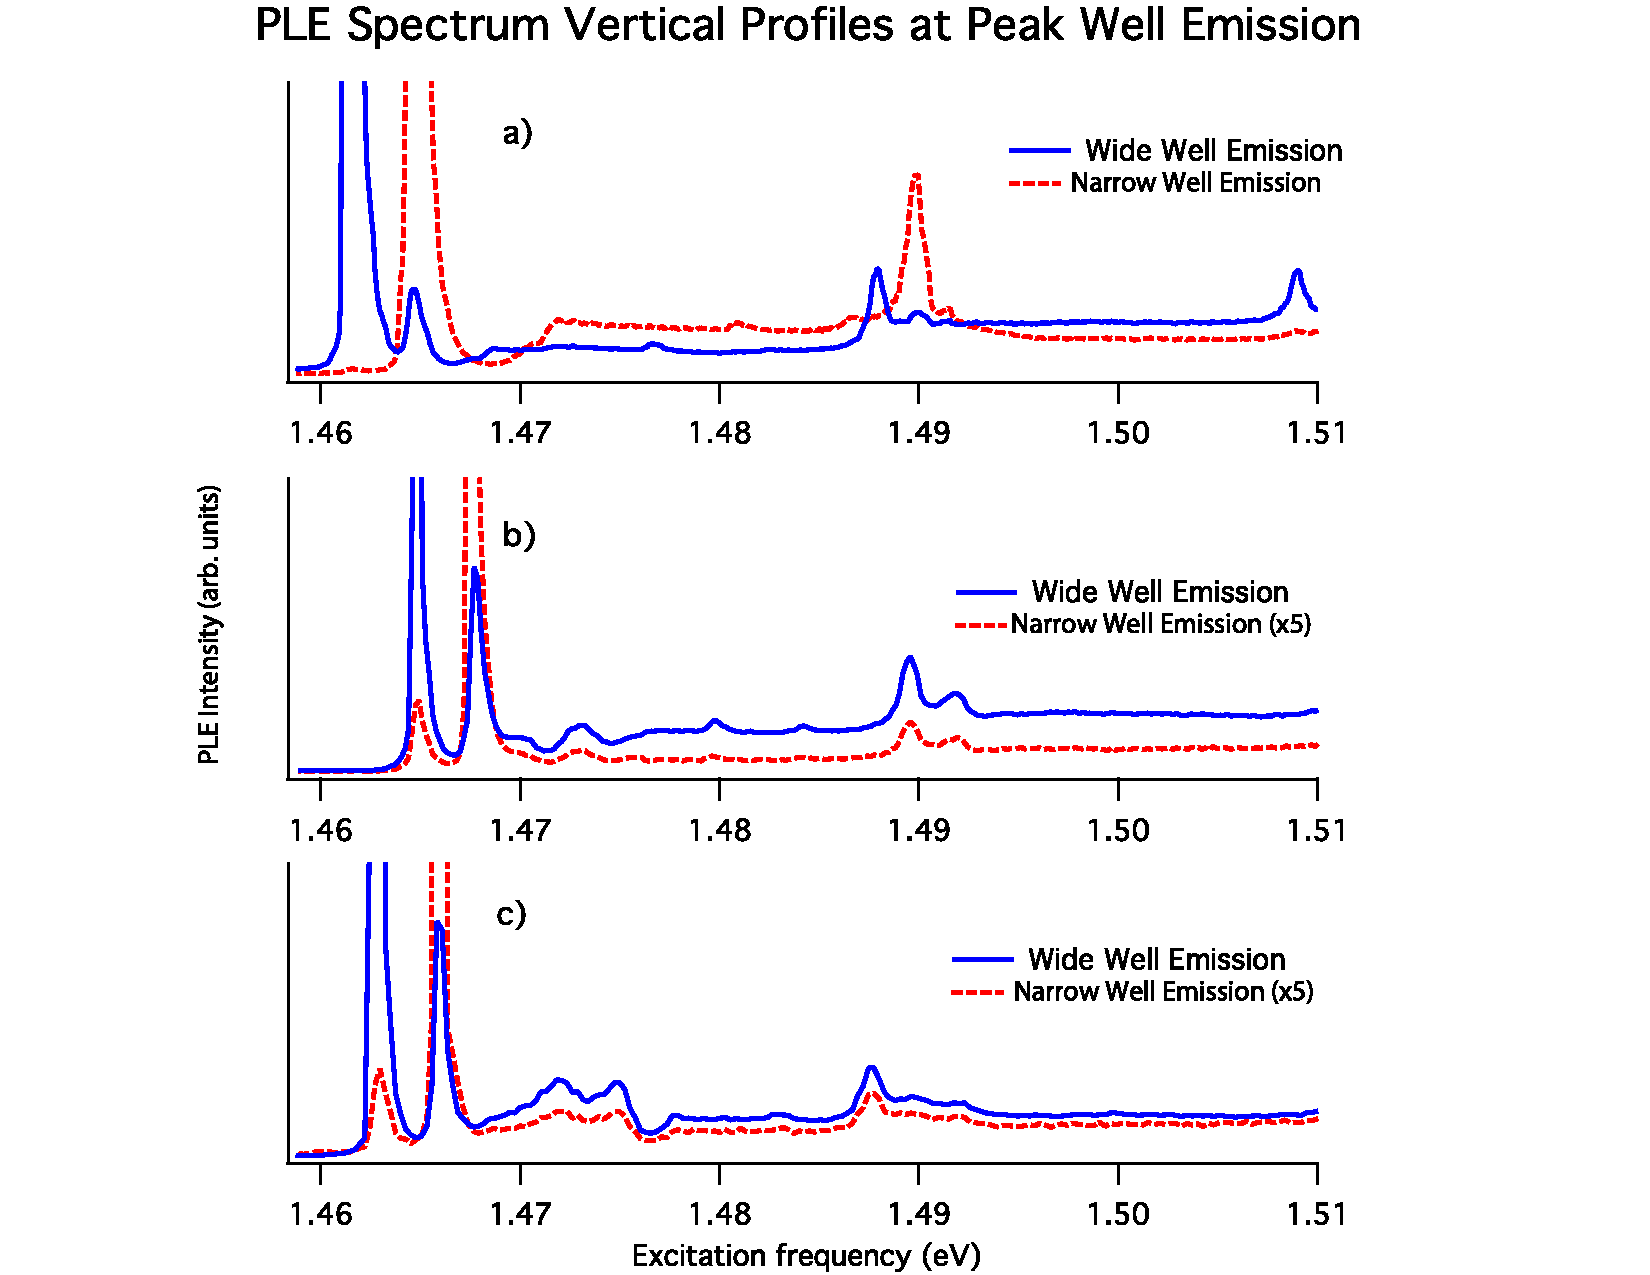
\includegraphics[width = 1.1\textwidth]{Layout2.pdf}
\caption{ \doublespacing A set of three PLE vertical profiles taken at the wavelength of peak emission intensity for a) the 30nm, b) the 10nm, and c) the 5nm barrier width AQW. Note: the narrow well emission intensity was much lower than the wide well emission intensity, and was scaled up for graphical comparison. For each sample, the most intense peaks correspond to resonant excitation and absorption. The coupling intensity can be measured by looking at the intensity of the cross peaks, represented by the slightly smaller peaks under each of the resonant excitation peaks.} 
\label{traces}
\end{figure}
\begin{figure}
\centering
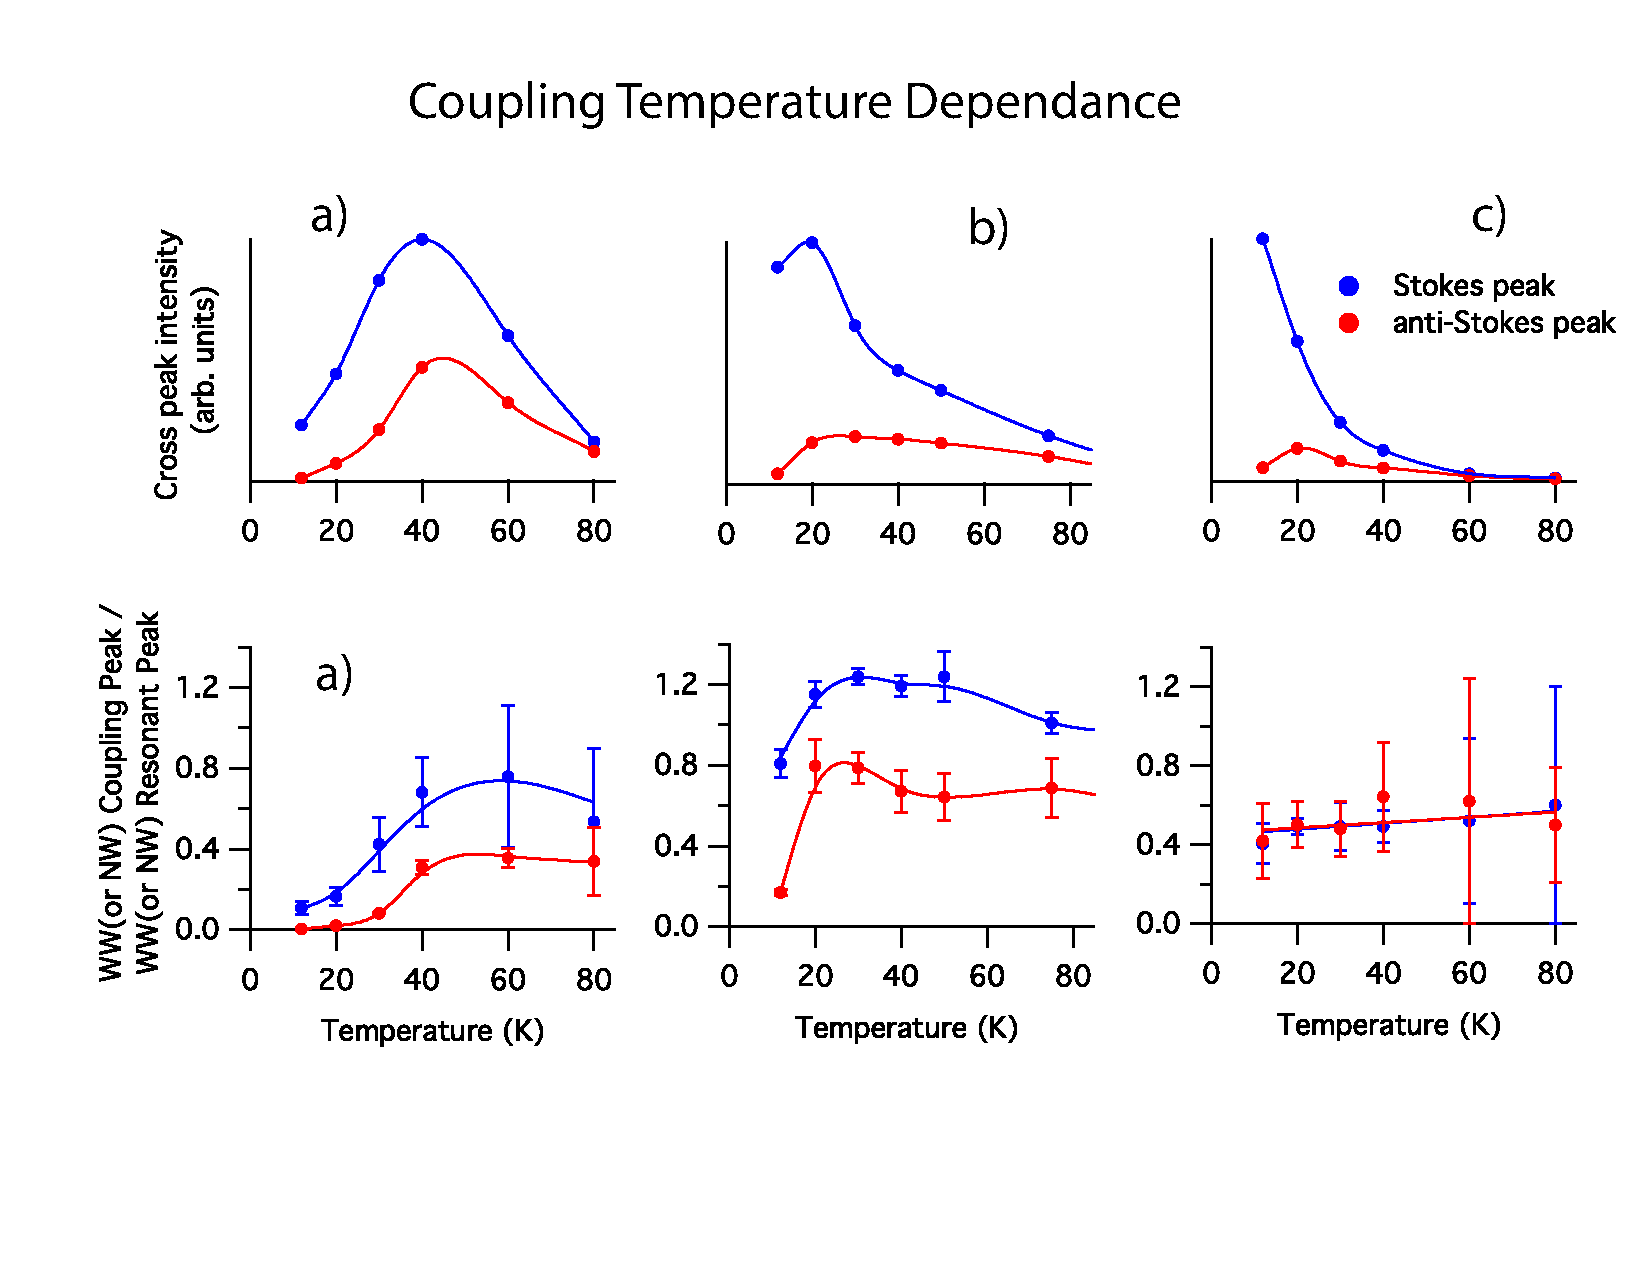
\includegraphics[width = \textwidth]{Layoutple2.pdf}
\caption{ \doublespacing Temperature dependance for the PLE coupling peaks for barrier width of a) 30nm, b) 10nm, and c) 5nm. The top plots are un-normalized coupling peak intensities, while in the bottom plots, the cross-peak intensity is normalized to the resonant peak intensity. The coupling intensity seems to peak have a temperature peak for the 30nm and 10nm barrier samples. The coupling peak intensities in both the normalized and unnormalized plots for these two samples decrease as sample temperature increases, suggesting that coupling is temperature mediated. However, in the 5nm barrier, there seems to be little temperature dependance of coupling intensity in the normalized plot.} 
\label{xpkintensity}
\end{figure}
%\begin{itemize}
%\item PLE curve analysis\\
%show stock PLE curve, show slices, say what they mean, show peaks, say what peaks mean
%\item PLE anti-Stokes.
%show anti-Stokes t dep. curves\\
%show anti-Stokes pow-dep curves, talk about linearity or no, comment on CCD bs., \\
%compare with thry, talk about mechanisms. well width dep
%\item PLE Stokes peak\\
%show Stokes pow-dep curves, talk about linearity or no, comment on CCD bs., \\
%compare with thry, talk about well width dep, say mechanisms understood(?) point to lit chris and I found
%\end{itemize}
